\documentclass[a4paper]{article}
\usepackage[BoldFont, SlantFont, CJKchecksingle]{xeCJK}
\usepackage{hyperref}
\usepackage{minted}
\usepackage{amsmath}
%\usepackage[3D]{movie15}
%\usepackage{fp}
%\usepackage{media9}

%\usepackage{xcolor}
%\usepackage{listings}
%
%\lstdefinestyle{BashInputStyle}{
%language=bash,
%basicstyle=\small\sffamily,
%numbers=left,
%numberstyle=\tiny,
%numbersep=3pt,
%frame=tb,
%columns=fullflexible,
%backgroundcolor=\color{yellow!20},
%linewidth=1.0\linewidth,
%xleftmargin=0.1\linewidth
%}
%\newcommand*{\Package}[1]{\texttt{#1}}%

\setCJKmainfont[Mapping=tex-text]{WenQuanYi Micro Hei}
\setCJKsansfont[Mapping=tex-text]{WenQuanYi Micro Hei}
\setCJKmonofont[Mapping=tex-text]{WenQuanYi Micro Hei Mono}
\title{Accelerate Reed-Solomon Coding for Fault-Tolerance in RAID-like system}
%\author{袁帥}
\author{Shuai YUAN}
\date{}

\begin{document}
\maketitle

\section{Background}
\subsection{Why Reed-Solomon codes?}
In a RAID-like system, storage is distributed among several devices, the probability of one of these devices failing becomes significant. 
To be specific, if the MTTF (mean time to failure) of one device is $P$, then the mean time to failure of a system of $n$
devices is $\dfrac{P}{n}$. 
Thus in such systems, fault-tolerance must be taken into account.

One common approach for fault-tolerance is replication. However, when data size scales up, replication will result in large storage overhead.

Here comes another solution of erasure codes, which can reduce the redundancy ratio tremendously.
%Given the same data availability, erasure codes have less redundancy ratio than replication.
%The motivation of using erasure coding comes from the need to reduce the storage overhead.
And among various types of erasure codes, Reed-Solomon code is one of the popular that frequently used in research.

Reed-Solomon code is a kind of optimal erasure codes which has the so-called Maximum Distance Separable (MDS) property.
$(n, k)$ MDS property is defined as:
Given original data, we divide it into $k$ equal-size native fragments, and encode them into $n$ fragments.
Then we can select any $k$ out of $n$ fragments to reconstruct the original data. 
It provides good flexibility for reconstruction, and the storage overhead is low: let the size of the original data is $M$, then the storage overhead is only $(n-k)\dfrac{M}{k}$ since we have $(n-k)$ more fragments.

\subsection{Reed-Solomon coding mechanism}

Let $D = [d_{1}, d_{2}, \cdots, d_{k}]^{T}$ be the $k$ native data fragments, 
Reed-Solomon code has mainly two processes:
%, one for encoding and another for decoding:
\begin{itemize}
%In the encoding process, 
\item encoding process: 
a encoding matrix $V = [v(i,j)]_{k \times (n-k)}$
%which has MDS property, 
is used to produce $(n-k)$ code fragments $C = [c_{1}, c_{2}, \cdots, c_{(n-k)}]^{T}$:
$$
c_{j} = \sum_{i = 1}^{k} v(i,j) \cdot d_{i}
$$

To achieve MDS property,
Reed-Solomon code uses a particular encoding matrix,
which is a Vandermonde's Matrix $v(i,j) = i^{(j-1)}$,
and limit all arithmetic operations in Galois Field.

After completing code fragments generation, we store $(n-k)$ code fragments together with $k$ native fragments.

%In the decoding process, 
\item decoding process: 
we randomly select $k$ out of $n$ fragments, say $X = [x_{1}, x_{2}, \cdots, x_{k}]^{T}$.
Then we use the coefficients of each fragments $x_{i}$ to construct a $k \times k$ matrix $V'$.
Original data can be regenerated by multiplying matrix $X$ with the inverse of matrix $V'$:
\end{itemize}
$$
D = V'^{-1} X 
$$

\subsection{Optimization motivation}
The reason that discourages using Reed-Solomon coding to replace replication is its high computational complexity:
Galois Field arithmetic is complex, and matrix operations consume a lot of time. 

Our goal is to use GPU to accelerate Reed-Solomon encoding and decoding. Our code is written in CUDA.

\section{Data type and size}
Instead of implementing the Reed-Solomon coding above the bare storage system, 
I implement it upon the file system. 
leaving some issues like how to stripe the file into several devices to the file system and controller of storage system.
%How to stripe the file into several devices is not considered here.

For the input data, it must be a file. There is no special limitation for the type and size of the file.

\section{How to use CUDA to accelerate}

\subsection{Accelerate operations in Galois Field (GF)}

%%As stated in \cite{}
%A
%%Galois
%field GF(n) is a set of $n$ elements closed under addition and multiplication, for which
%every element has an additive and multiplicative inverse (except for the 0 element which
%has no multiplicative inverse). 

Operations in Galois Field is one of the bottlenecks in Reed-Solomon coding performance, thus deserving to find an appropriate way for GPU to accelerate.

As stated in \cite{sklar2001reed},
GF($2^w$) field is constructed by finding a primitive polynomial $q(x)$ of degree $w$ over GF(2), and then enumerating the elements (which are polynomials) with the generator $x$.
Addition in this field is performed using polynomial addition, and multiplication is performed using polynomial multiplication and taking the result modulo $q(x)$.

In implementation, we
map the elements of GF($2^w$) to binary words of size $w$
, so that computation in GF($2^w$) becomes bitwise operations.
Let $r(x)$ be a polynomial in GF($2^w$). Then we can map $r(x)$ to a binary word $b$ of size $w$ by setting the $i$th bit of $b$ to the coefficient of $x^i$ in $r(x)$.


After mapping, 
addition and subtraction of binary elements of GF($2^w$) can be performed by bitwise exclusive-or, which is fast. 

However, multiplication 
is still costly.
%
One must convert the binary numbers to their polynomial
elements, multiply the polynomials modulo $q(x)$, and then convert the answer back to binary.
%One traditional way to compute multiplication is through a loop of bit operations:
To compute the result of binary word $b$ multiplied by binary word $a$ in GF($2^w$),
we have to use bitwise operations to emulate polynomial of $b$ multiplying the polynomial of $a$ modulo $q(x)$.
Here shows how to perform byte multiplication in GF($2^8$):
\begin{minted}[frame=lines,mathescape]{c}
uint8_t gf256_mul_by_bit(uint8_t a, uint8_t b)
{
  uint8_t result;
  while(b)
  {
    if(b & 1)
    {
      //emulate polynomial addition
      result ^= a;
    }
    //primitive polynomial of GF(2^8):
    //x^8+x^4+x^3+x^2+1
    //which is mapped into 0x1d
    //(a & 0x80? 0x1d: 0): emulate polynomial modulo
    a = (a << 1) ^ (a & 0x80? 0x1d: 0);
    b >>= 1;
  }
  return result;
}
\end{minted}

Such a loop takes at most 8 iterations to complete.
In Reed-Solomon coding, multiplication in GF($2^w$) is used so frequently that such cost is unbearable.


Another approach is to store all the result in a multiplication table.
which is adopted in CPU-based implementation 
like NCCloud \cite{hu2012nccloud}.

The multiplication table may use 
the bitwise method
mentioned above 
to setup at the beginning, or simply defined as constant. 

Again taking GF($2^8$) for instance, we setup the following table:
\begin{minted}[frame=lines]{c}
uint8_t  gf256mul[256][256];
\end{minted}
Here gf256mul[a][b] stores the result of binary word $b$ multiplied by binary word $a$.
Therefore, when computing multiplication, we simply need to find the corresponding item in the multiplication table.
Such an approach can speed up computation while sacrificing more memory space.

For a large-width finite field, 
this method might not be suitable for GPU.
%GPU has great computation power and memory access can be another bottleneck.
GPU has greater computation power than CPU, but memory access can be another bottleneck. One common optimization technique is to allocate shared memory space for the multiplication table.
But in GF($2^8$),
the multiplication table has $256 \times 256$ items, which consumes so large space that shared memory may not be able to provide.
In addition, note that $a \times b = b \times a$, there are redundancies in the multiplication table (e.g. gf256mul[a][b] is the same as gf256mul[b][a]), which is a waste of space.

However, this approach can still be applied in a field with smaller width,
and we have implemented it in GF($2^4$).
We use the multiplication table with $16 \times 16$ items and two helper tables(exponential and logarithm tables, will be introduced later) with $16$ items correspondingly for the convenience of div and pow operations. 
These tables are stored in the Constant Memory of GPU, which will be cached.
Since a byte is the smallest addressable unit, we need to transfer byte operations into multiple nibble (4-bit) operations.
(Note that simply extending 4bits to 8bits is not appropriate, since it is equivalent to doubling the file size and will increase the execution time.)
Here shows how we perform byte multiplication in GF($2^4$):
\begin{minted}[frame=lines]{c}
__host__ __device__ uint8_t gf_mul(uint8_t a, uint8_t b)
{
	uint8_t a_high_nibble = ( a >> 4 ) & 0x0f;
	uint8_t b_high_nibble = ( b >> 4 ) & 0x0f;
	uint8_t result_high_nibble = gfmul_16[a_high_nibble][b_high_nibble];
	uint8_t a_low_nibble = a & 0x0f;
	uint8_t b_low_nibble = b & 0x0f;
	uint8_t result_low_nibble = gfmul_16[a_low_nibble][b_low_nibble];

	return ( (result_high_nibble << 4) | result_low_nibble);
}
\end{minted}

For a large-width finite field, 
we need to make a trade-off between computation and memory: 
we still need to use shared memory to accelerate,
without produce much memory overhead like the multiplication table method.
Here comes the third approach \cite{plank1997tutorial}:


%Multiplication is a little more difficult. One must convert the binary numbers to their polynomial
%elements, multiply the polynomials modulo $q(x)$, and then convert the answer back to binary.
%This can be implemented, in a simple fashion, by using the two logarithm tables described
%earlier: one that maps from a binary element $b$ to power $j$ such that $x^j$
%is equivalent to $b$
%(this is the gflog table, and is referred to in the literature as a ‘discrete logarithm’), and one that
%maps from a power $j$ to its binary element $b$. Each table has $2^w$
%1 elements (there is no $j$ such that $x^j = 0$). Multiplication then consists of converting each binary element to its discrete
%logarithm, then adding the logarithms modulo $2^w-1$ (this is equivalent to multiplying the
%polynomials modulo $q(x)$) and converting the result back to a binary element. Division is performed in the same manner, except the logarithms are subtracted instead of added. Obviously,
%elements where $b = 0$ must be treated as special cases. Therefore, multiplication and division of two binary elements takes three table lookups and a modular addition.


%Trade-off:
%we build up smaller reference tables and store them in the shared memory.
%
%we use logarithm and exponential tables:

We build up two smaller tables:
\begin{itemize}
  \item exponential table: maps from a binary element $b$ to power $j$ such that $x^j$ is equivalent to $b$.
  \item logarithm table: maps from a power $j$ to its binary element $b$ such that $x^j$ is equivalent to $b$.
\end{itemize}
Multiplication in GF($2^w$) then consists of 
looking each binary number in the logarithm table for its logarithm (this is equivalent to finding the polynomial), 
then adding the logarithms modulo $2^w-1$ (this is equivalent to multiplying the polynomial modulo $q(x)$) 
and 
looking up exponential table to convert the result back to a binary number.
Here is the pseudo code for multiplication in GF($2^8$):
\begin{minted}[frame=lines,mathescape]{c}
//number of elements in GF(2^8)
int NW = 1 << 8;
uint8_t gf_mul(uint8_t a, uint8_t b)
{
  int result;
  if (a == 0 || b == 0)
  {
    return 0;
  }
  result = (gflog[a] + gflog[b]) % (NW-1);
  return gfexp[result];
}
\end{minted}
Division is performed in the same manner, except the logarithms are subtracted instead of added.

In this method, multiplication and division of two binary elements takes three table lookups and a modular addition,
which achieves better compromise for GPU.

\subsection{Accelerate encoding process}

Firstly, we need to generate a MDS encoding matrix,
which is a Vandermonde's Matrix in Reed-Solomon coding algorithm.
%$n$ row and $k$ column
%
%$$
%V(i, j) = i^{(j-1)}
%$$
This can be paralleled in GPU by letting every thread compute few items of Vandermonde's Matrix.
Since the power operations in GF($2^w$) is mapped to
%access some table entry,
table entry lookup and memory access,
the workload of all the threads is balanced.
%%%%%%%%%%
%Mark as ToDo
% While GPU is computing the encoding matrix, CPU can load the input file(s) into memory,
% thus making the IO and computation processing roughly at the same time.
%%%%%%%%%%

%Reed-Solomon encoding process is a 
Matrix multiplication to generate code fragments is the most suitable part for CUDA to accelerate.
Some common techniques like tile algorithm are used to optimize the computation/communication ratio.
%Here I use some common techniques like tile algorithm to optimize the computation/communication ratio.
Tile algorithm is used to improve the temporary locality and reduce cache misses when an array is accessed in a row major order and in a column major order at the same time (Matrix multiplication is such a good example). This technique is introduced in the classical computer architecture textbook \cite{hennessy2012computer} as \textbf{blocking}. For further details of the technique, please refer to \cite{nvidia2010cuda}.

\subsection{Accelerate decoding process}

In the decoding process of Reed-Solomon coding, 
we read arbitrary $k$ out of $n$ fragments to reconstruct and the total time of read access is as fast as the response time of the slowest storage node.
%to respond to reading of the corresponding fragments.
%Therefore, 

%%%%%%%%%%
%Mark as ToDo
% To avoid the effect of some slow storage node,
% we perform aggressive read:
% read all $n$ fragments,
% and when there are $k$ fragments completing IO ,
% we complete the read request and use the first $k$ fragments to decode.
%%%%%%%%%%

%we need to compute the inverse of the encoding matrix, and then multiply it by $k$ out of $n$ fragments to reconstruct the original data.

After knowing which $k$ fragments are used for decoding, we know the corresponding rows of coefficients in the encoding matrix $V$.
These rows form the $k \times k$ matrix $V'$, and we need to compute its inverse.
Unfortunately, we found no standard APIs for inversing a matrix in Galois Field, 
%and modifying source code
so we implement Gauss elimination to compute inverse matrix: 
augment the square matrix $V'$ with the identity matrix $I$ of the same dimensions to obtain $[V' | I]$ and then apply matrix operations to transfer $[V' | I]$ into its reduced row echelon form: $V'^{-1}[V' | I] = [I | V'^{-1}]$.

Gauss elimination contains the following steps:
\begin{enumerate}
\item Check whether the diagonal item in the current row of $V'$ is nonzero. If if is zero, find a nonzero item and switch the two columns. The same column switching should also apply to $I$. Then the diagonal item in the current row of $V'$ is our pivot.
\item Normalize the current row by the pivot.
\item Eliminate other rows so that the reverse column of the the current row becomes reduced echelon form.
\end{enumerate}
Step 2 and Step 3 are suitable for GPU to parallely execute, but since we have to set barriers between steps, Gauss elimination is still not a fully-paralleled algorithm.

Finally, we multiply matrix $V'^{-1}$ with the matrix of $k$ fragments,
and the original data is reconstructed. This part is the same as the matrix multiplication in the encoding process.

\section{Experiment Result}
%\subsection{CPU vs GPU}
Experiment Setting:
\begin{itemize}
  \item CPU: Intel(R) Xeon(R) CPU E5620  @ 2.40GHz
  \item GPU: nVidia Corporation GF100 [Tesla C2050]
  \item nVidia Corporation GF100 [Tesla C2050]
	\begin{itemize}
	  \item 448 CUDA cores @ 1.15GHz
	  \item 3GB GDDR5 (1.44GB/s)
	  \item 64KB L1 cache + shared memory / 32 cores, 768KB L2 cache
	\end{itemize}
%  \item k=4, n=6 for GPU vs CPU
%  \item $k=4, n=6$
\end{itemize}

\subsection{GPU Cost Breakdown}

In this experiment, we set $k=4, n=6$.

The following figure shows the time of GPU encoding progress steps.

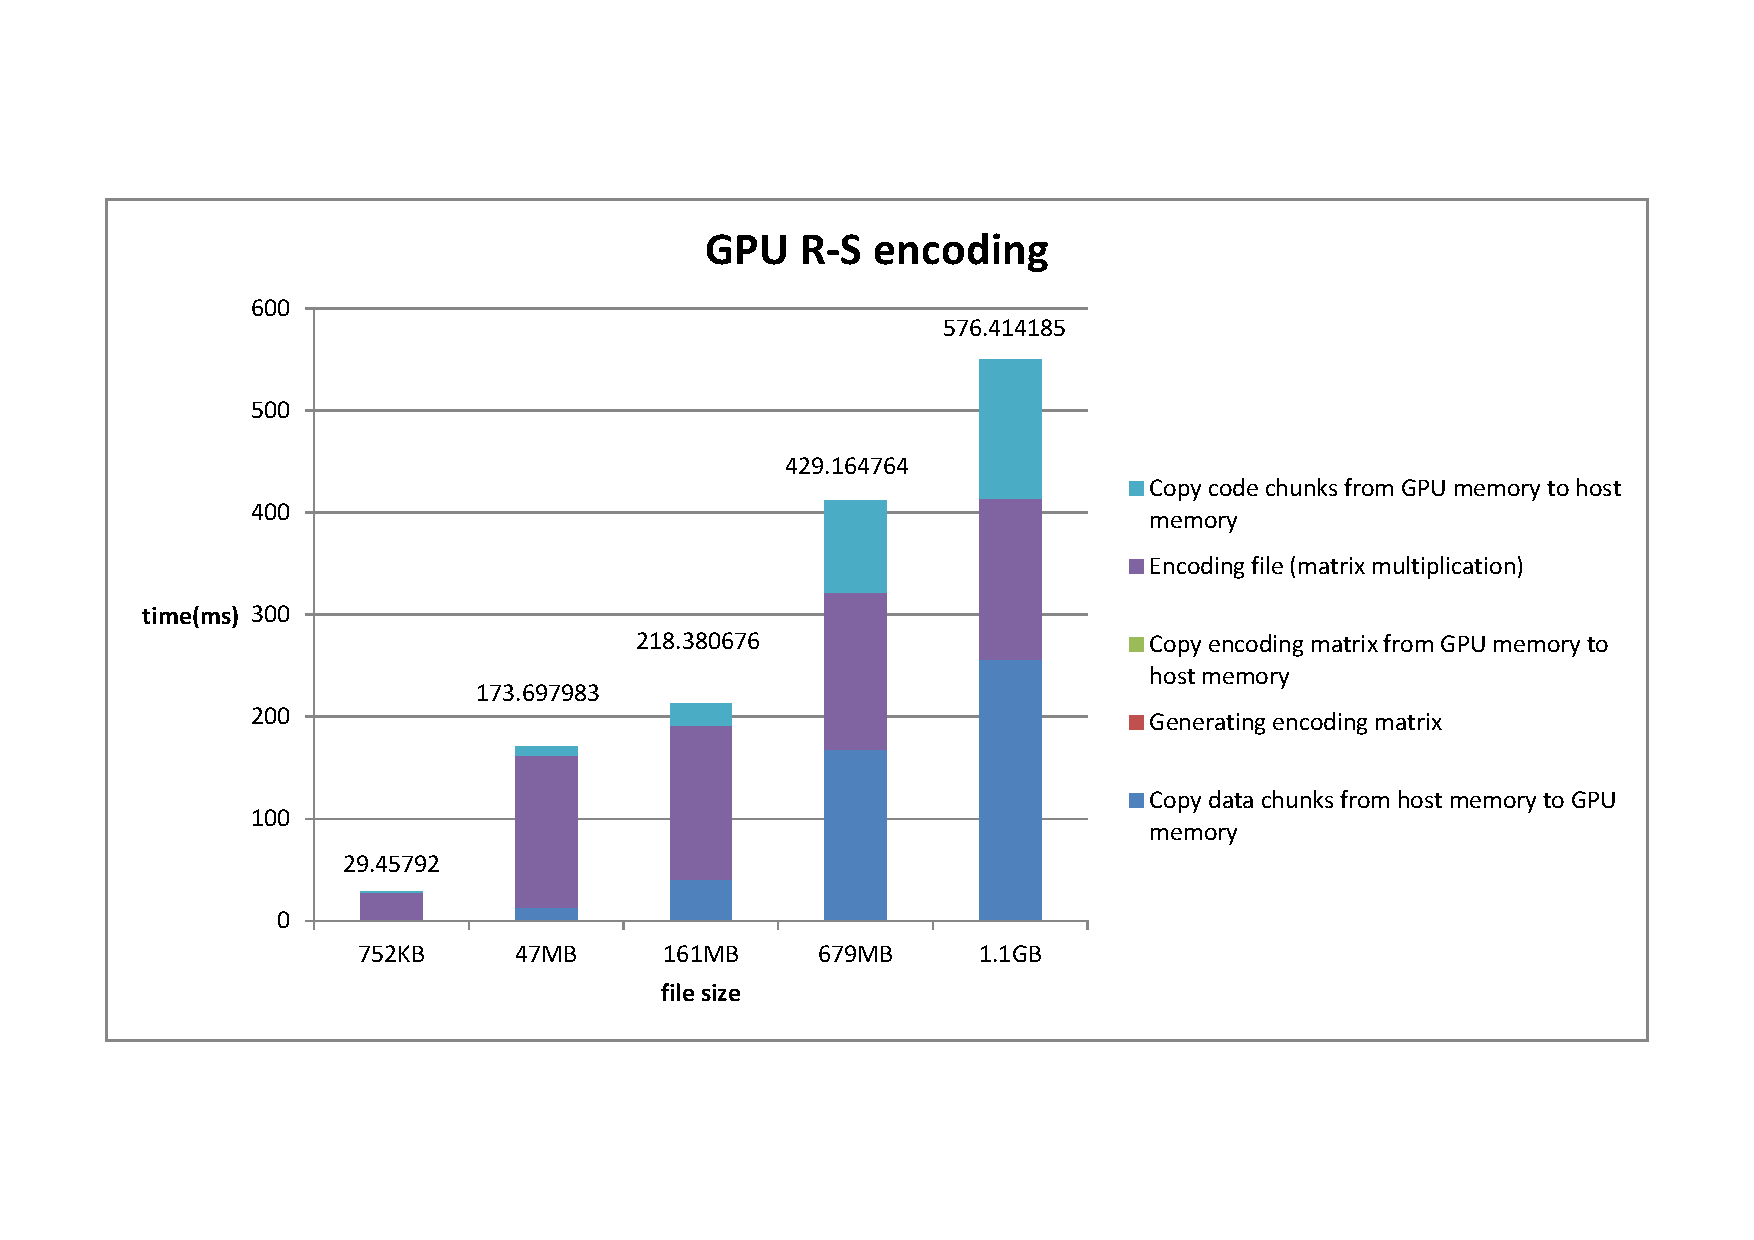
\includegraphics[scale=0.48]{result-graph/GPU-encode-steps.pdf}

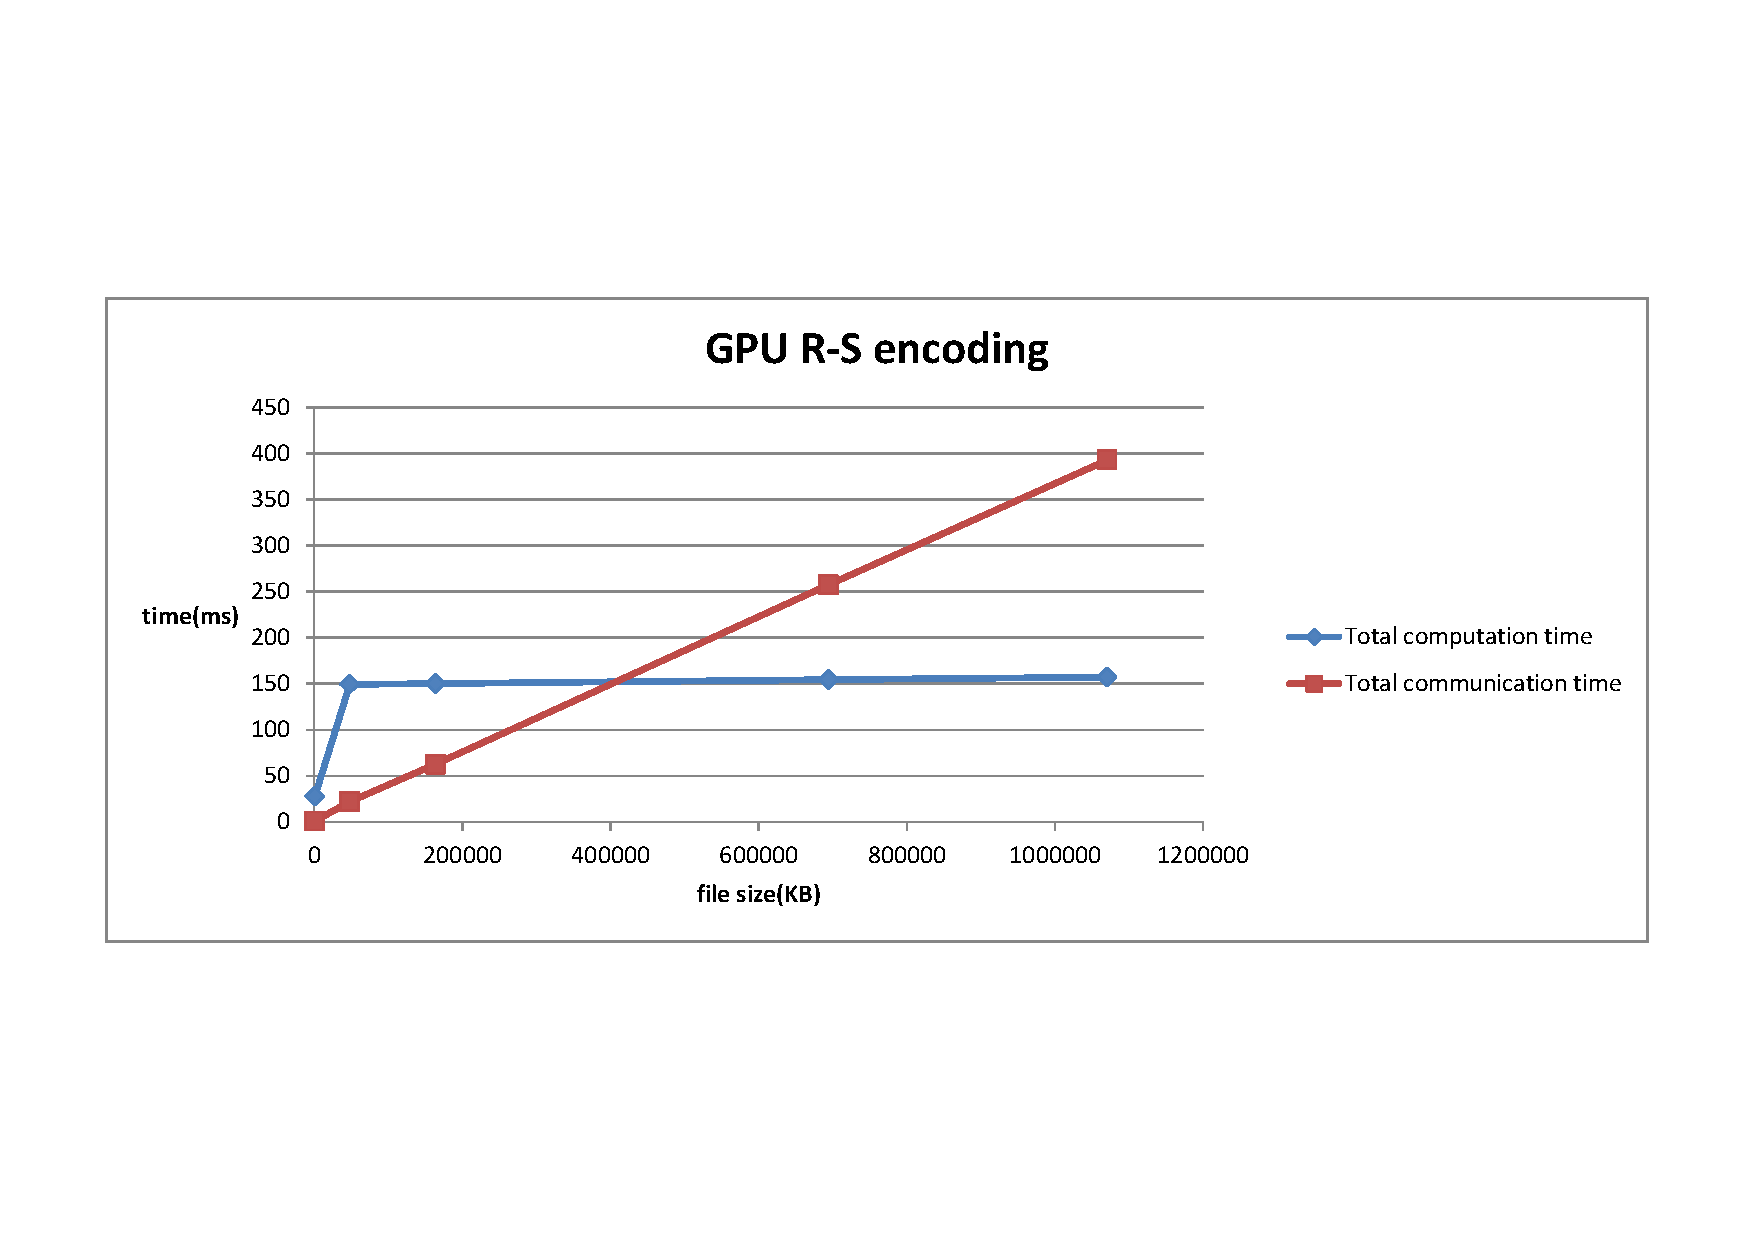
\includegraphics[scale=0.42]{result-graph/GPU-RS-encode.pdf}

The following figure shows the time of GPU decoding progress steps.

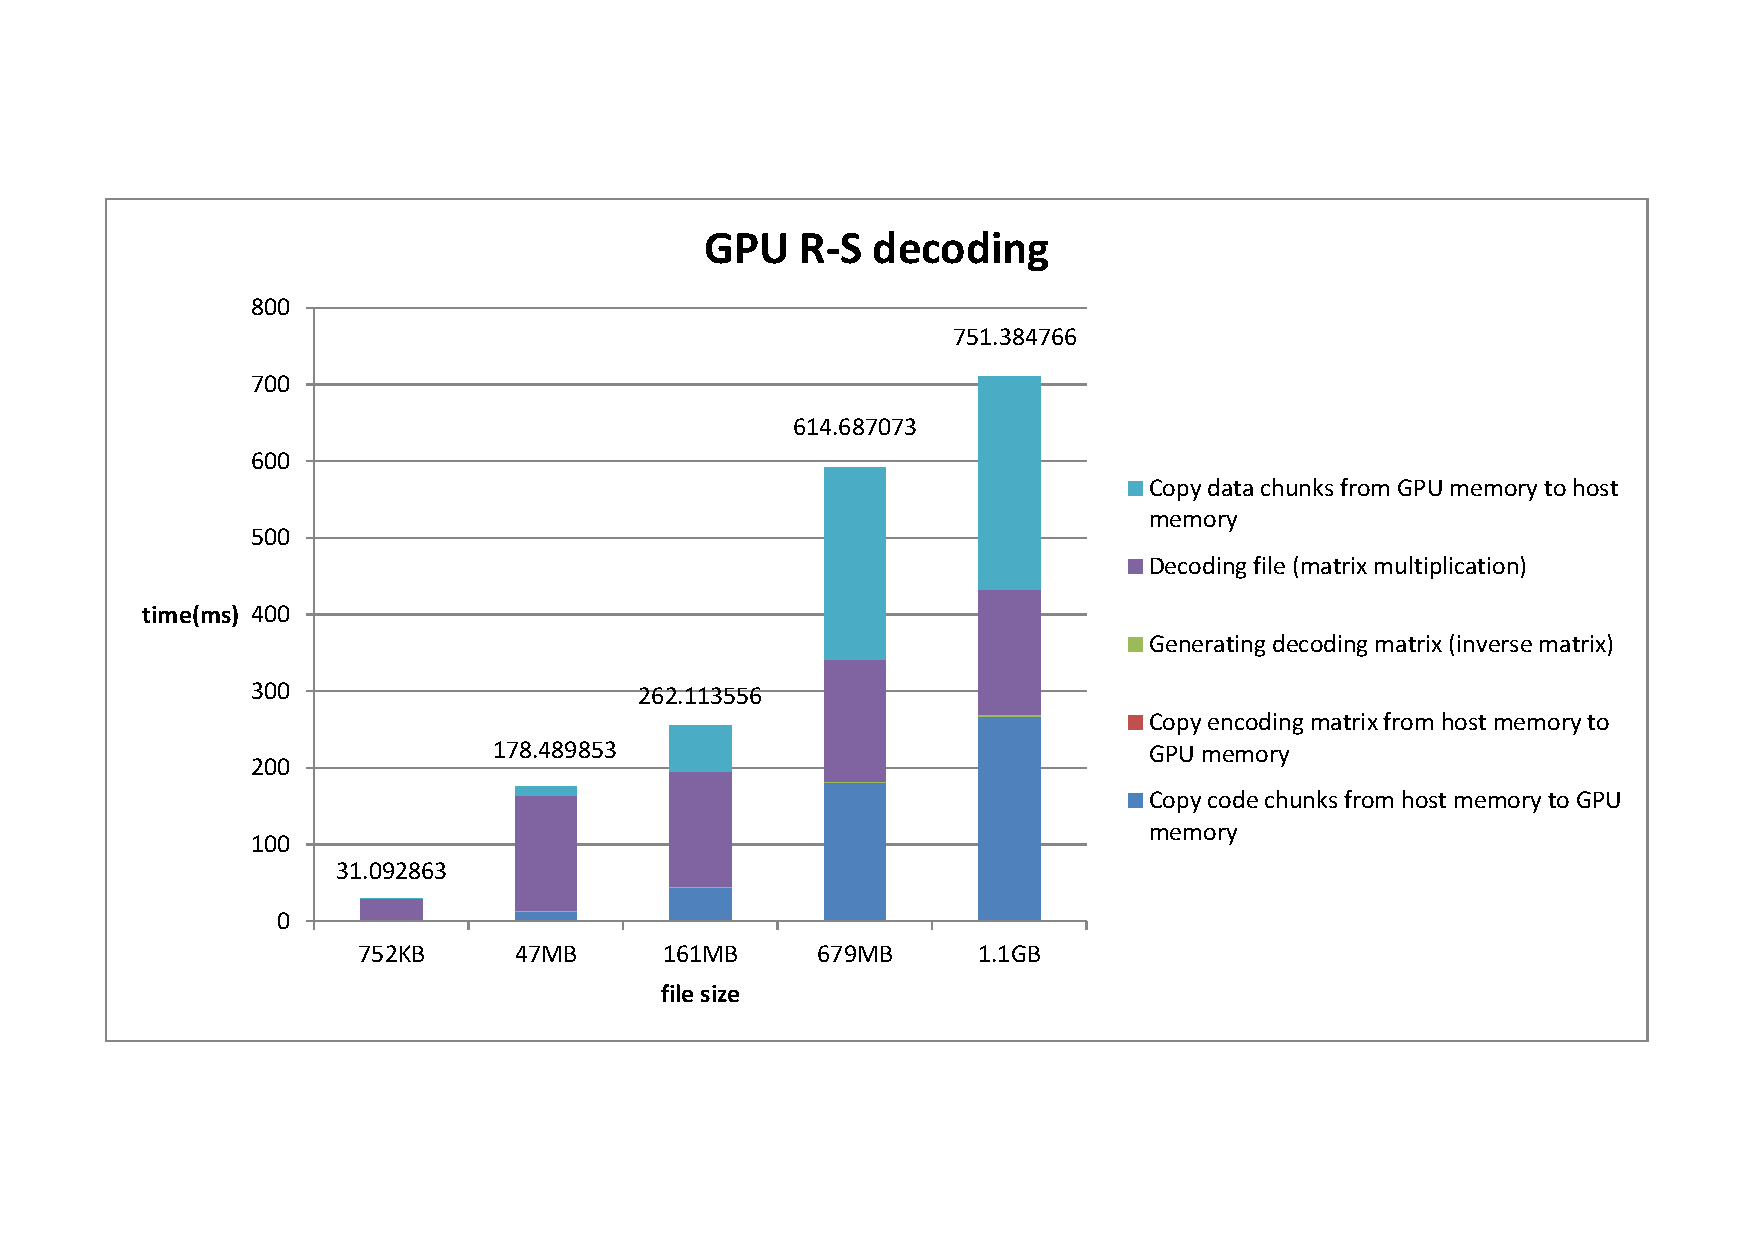
\includegraphics[scale=0.48]{result-graph/GPU-decode-steps.pdf}

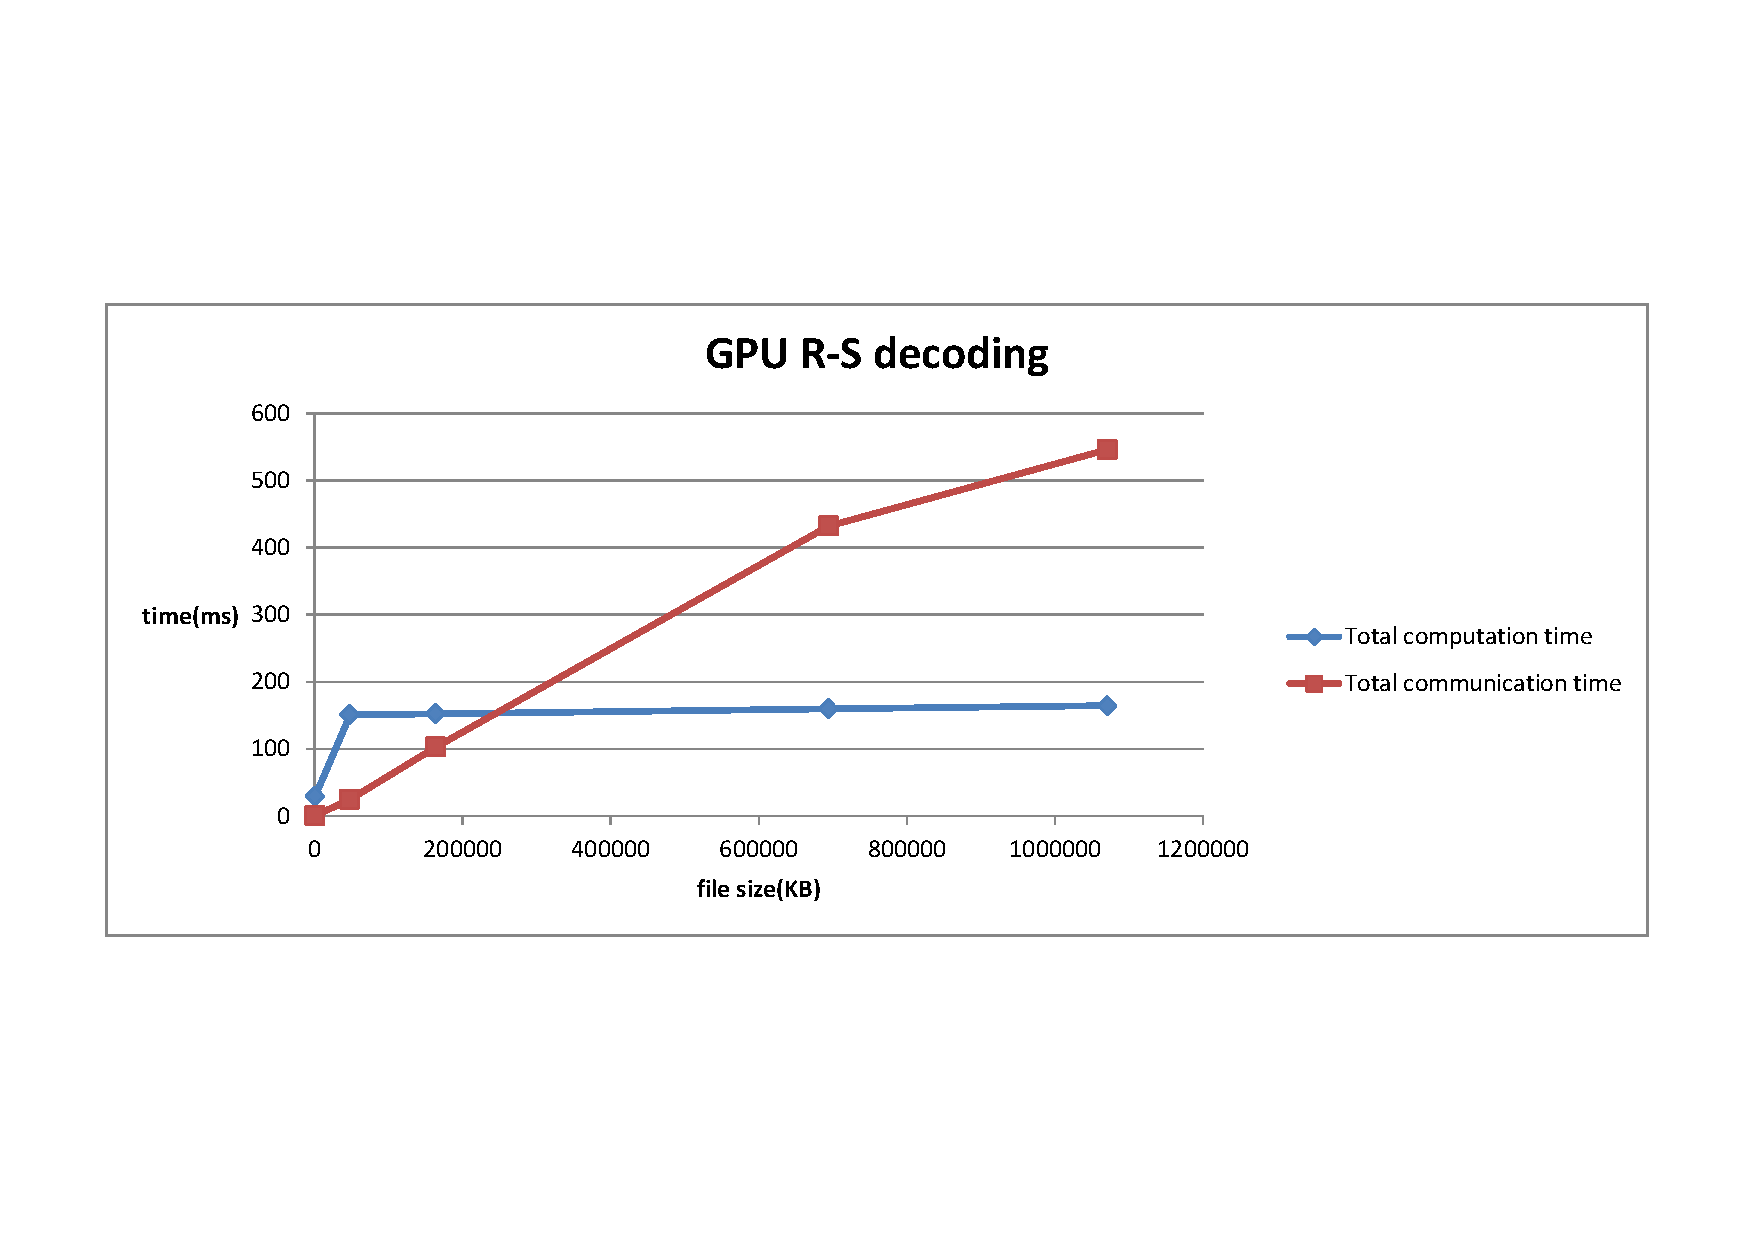
\includegraphics[scale=0.42]{result-graph/GPU-RS-decode.pdf}

Conclusion:
\begin{enumerate}
\item GPU computation time becomes almost constant when the file size is large enough.
\item Matrix multiplication time occupies much more percentage than matrix generation time in the breakdown of GPU computation time.
\item GPU spends more time in communication and the communication time is getting more as the file size becomes larger. This phenomenon explains why GPU performance speed-up gets slower.
\end{enumerate}

\subsection{CPU vs GPU}

We set $k=4, n=6$, the same as the above experiment.

The following figure shows the bandwidth comparison between CPU and GPU in the Reed-Solomon encoding progress.

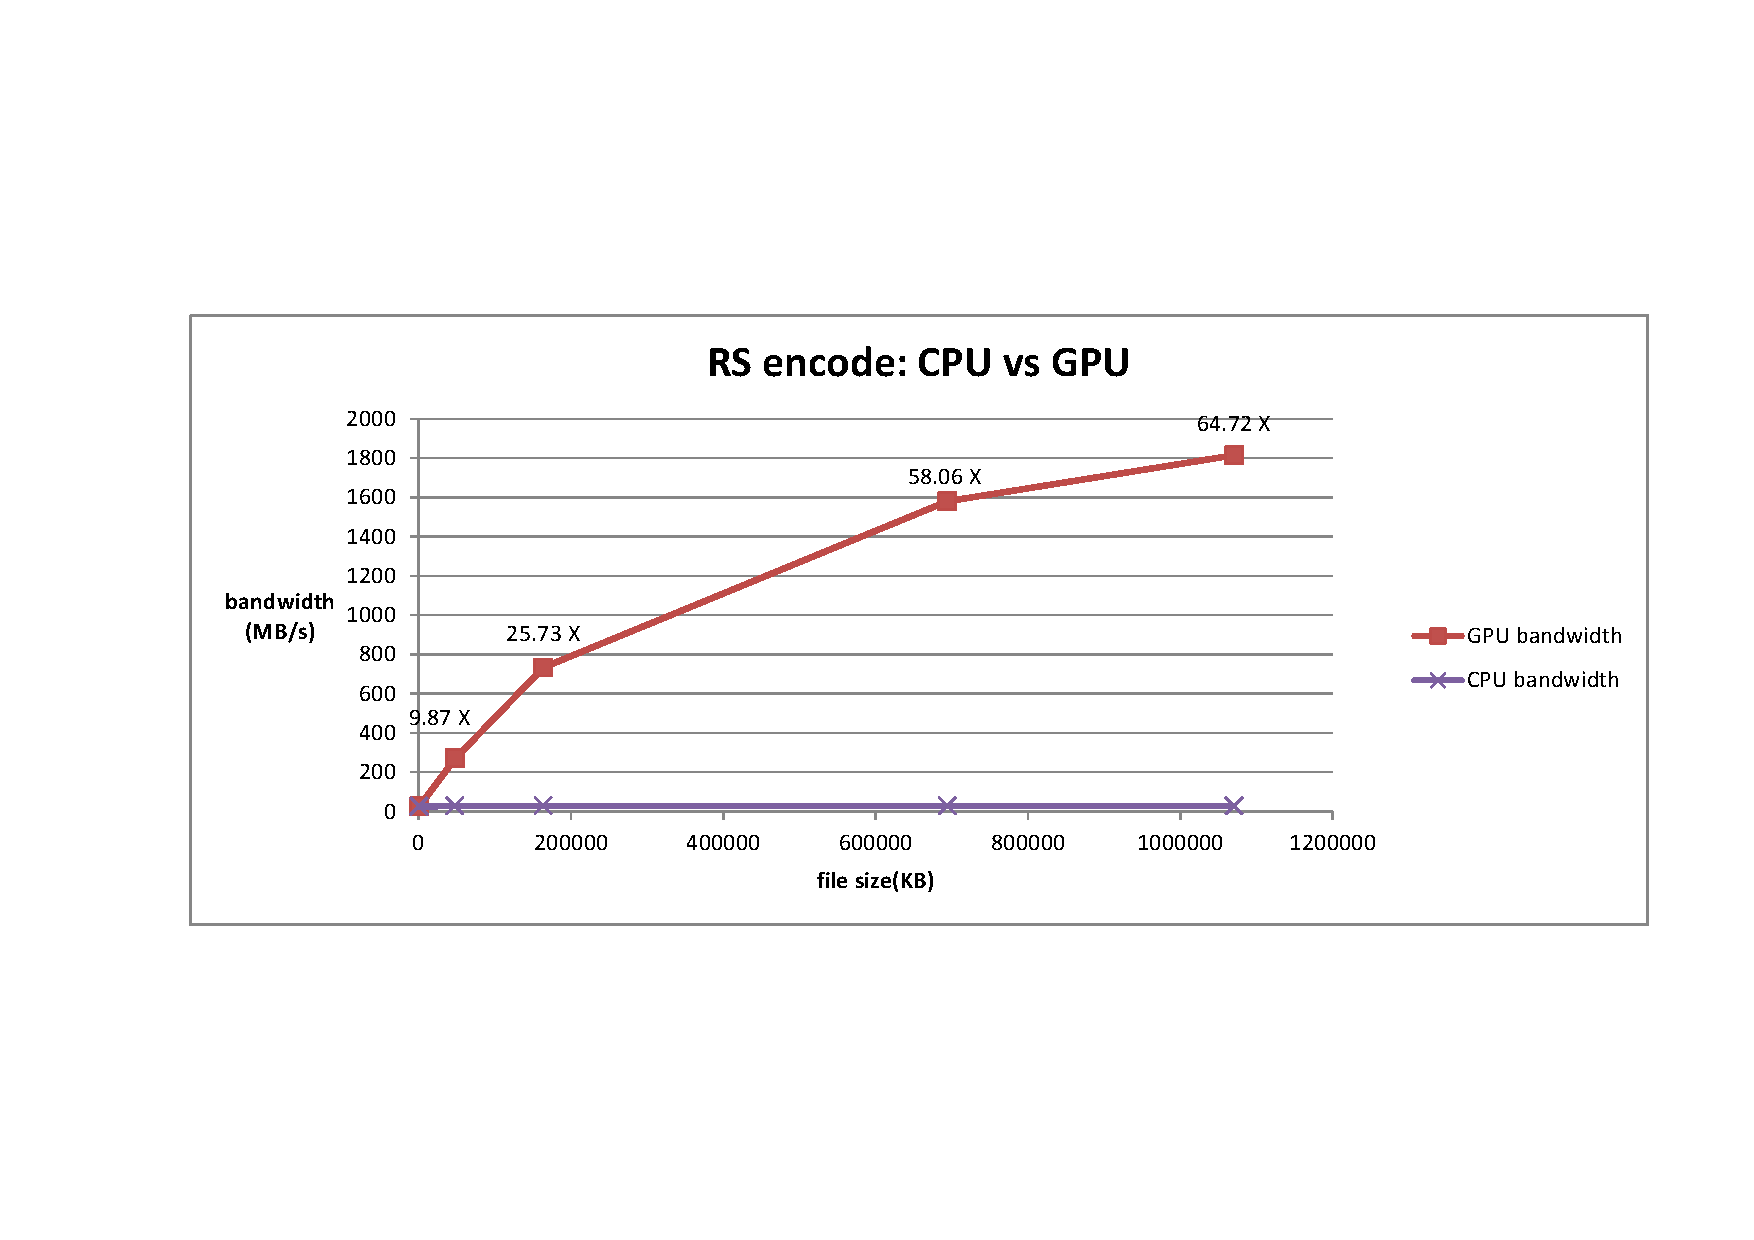
\includegraphics[scale=0.48]{result-graph/encode-CPU-vs-GPU-graph.pdf}
Table \ref{encoding-speed-up} is the performance speed-up of GPU in the Reed-Solomon encoding progress:
\begin{table}
\caption{
GPU speed-up in the Reed-Solomon encoding progress
}
\begin{center}
\begin{tabular}{|c|c|c|c|c|c|}
\hline
size(Byte) &  752 & 47968 & 163864 & 694276 & 1070616 \\
\hline
speed-up   &  -   & 9.87  & 25.73  & 58.06  & 64.72 \\
\hline
\end{tabular}
\label{encoding-speed-up}
\end{center}
\end{table}

The following figure shows the bandwidth comparison between CPU and GPU in the Reed-Solomon decoding progress.

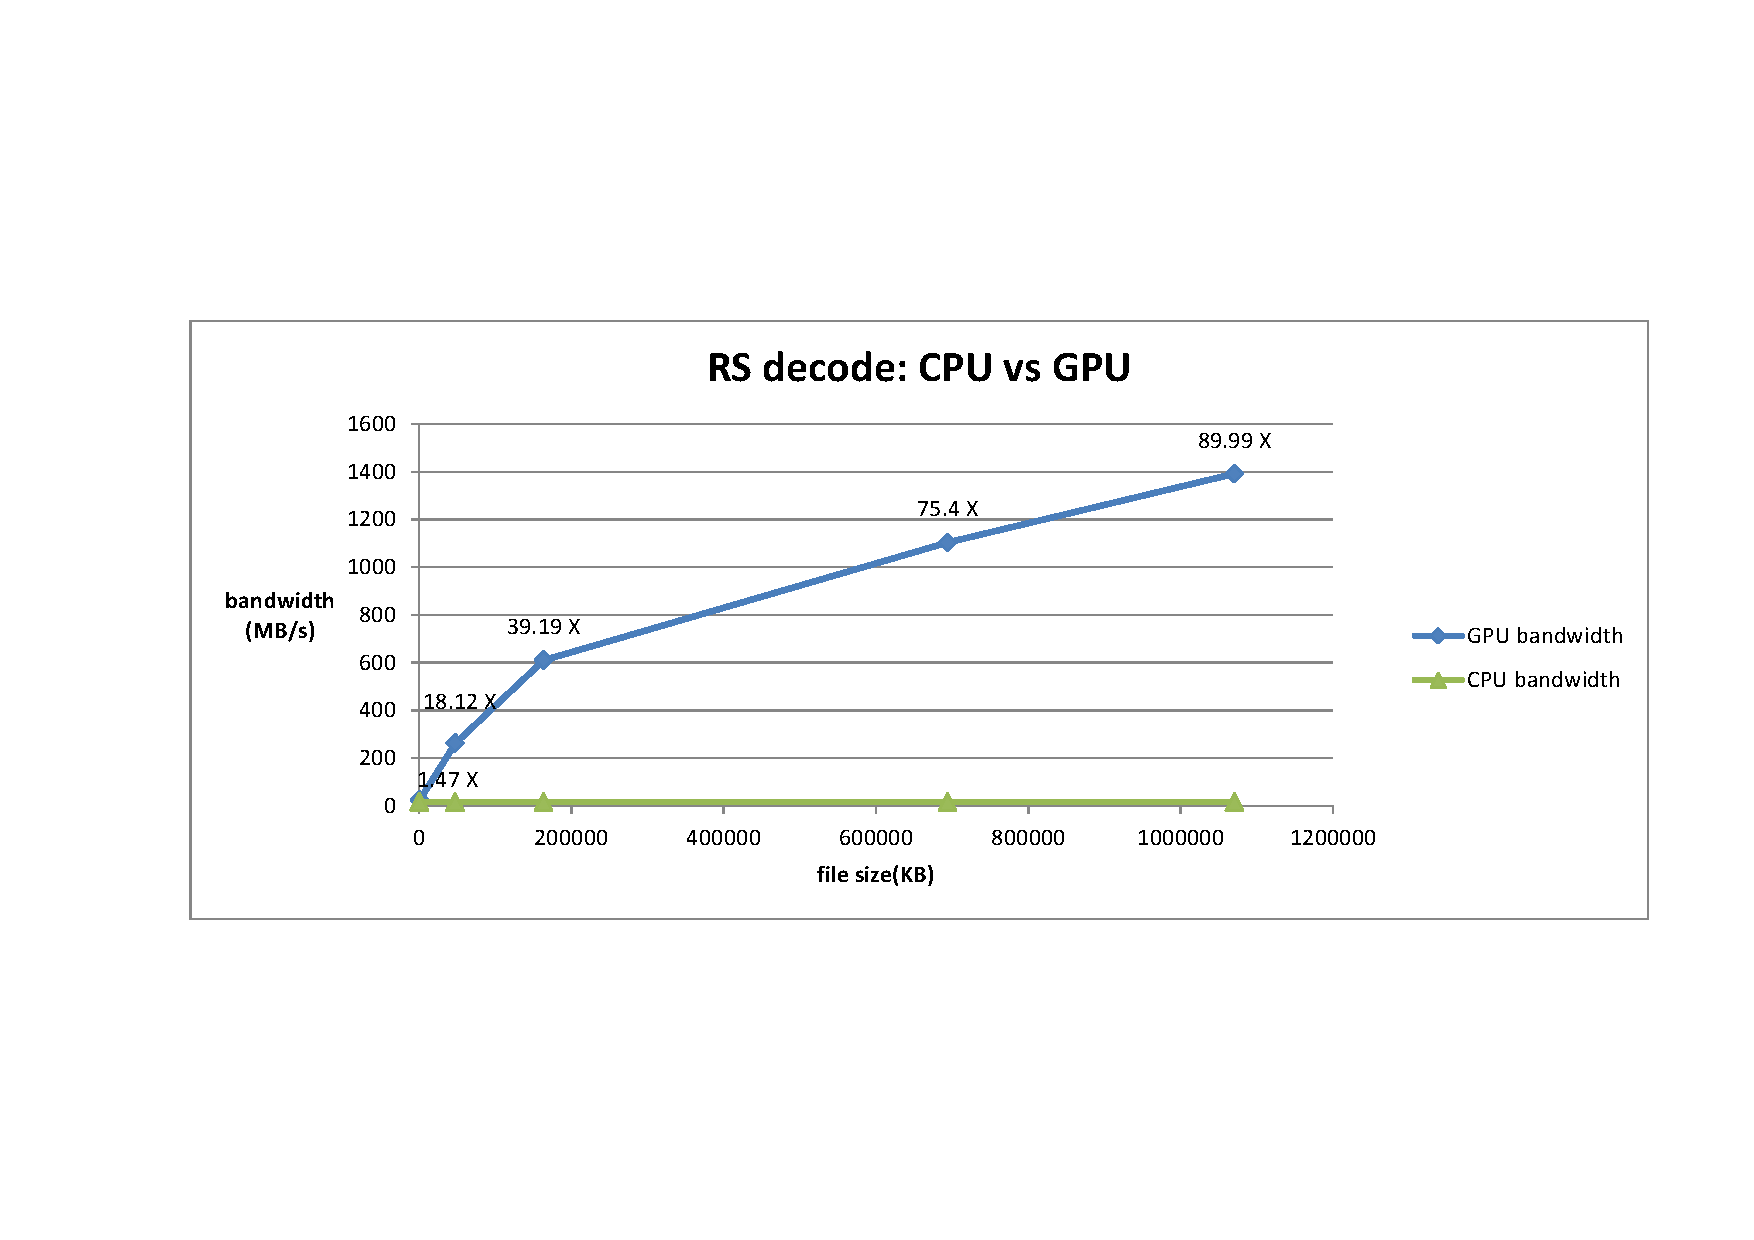
\includegraphics[scale=0.48]{result-graph/decode-CPU-vs-GPU-graph.pdf}
Table \ref{decoding-speed-up} is the performance speed-up of GPU in the Reed-Solomon encoding progress:
\begin{table}
\caption{
GPU speed-up in the Reed-Solomon decoding progress
}
\begin{center}
\begin{tabular}{|c|c|c|c|c|c|}
\hline
size(Byte) & 752  & 47968 & 163864 & 694276 & 1070616 \\
\hline
speed-up   & 1.47 & 18.12 & 39.19  & 75.4   & 89.99 \\
\hline
\end{tabular}
\end{center}
\label{decoding-speed-up}
\end{table}

Conclusion:
\begin{enumerate}
\item CPU bandwidth is nearly constant.
\item GPU achieves better speed-up when the file size scales up.
\item GPU performance speed-up gets slower.
\end{enumerate}

%\subsection{Tuning k}

Since double and triple fault tolerance is the most commonly used, we treat $k$ as a variable with fixed file size of 1.1GB and run several experiments in these two cases.

For double fault tolerance:

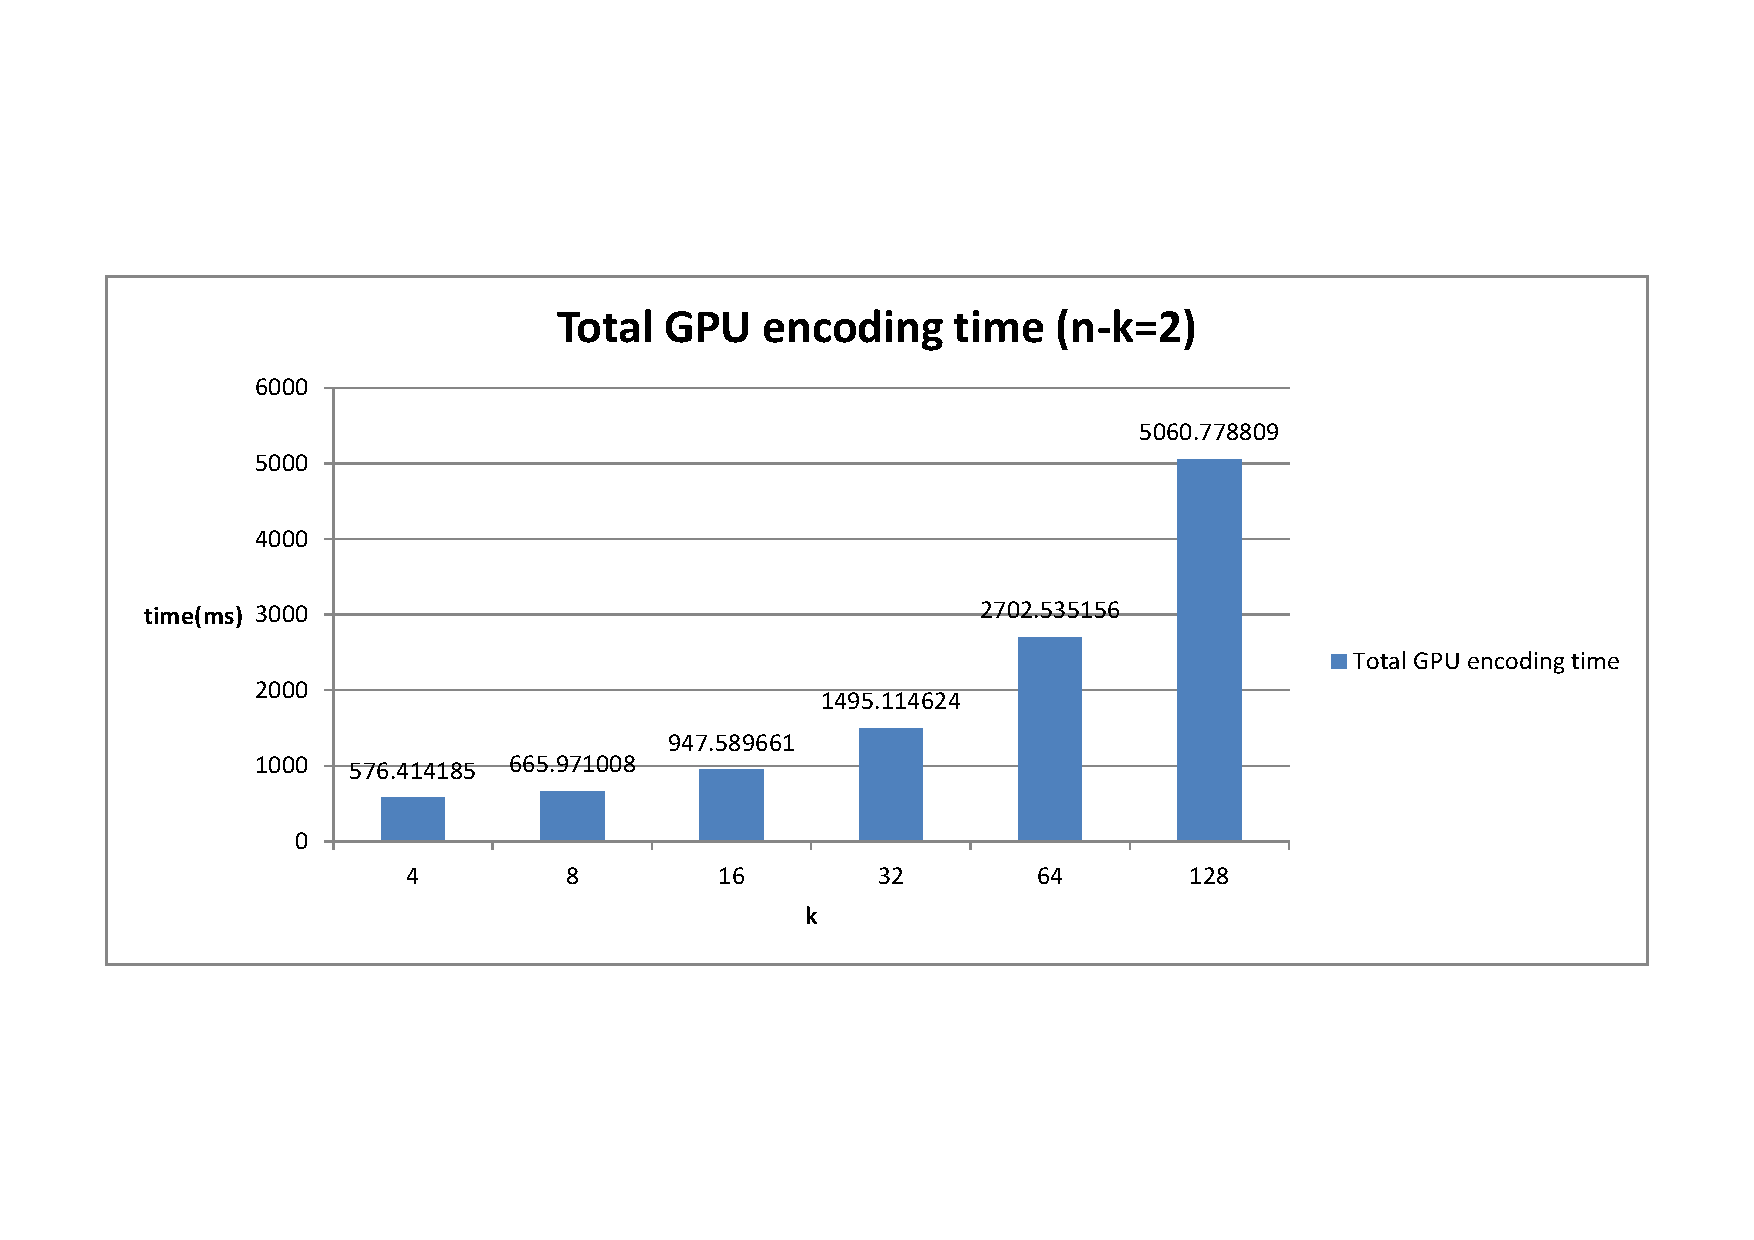
\includegraphics[scale=0.5]{result-graph/Total-GPU-encoding-time-2.pdf}

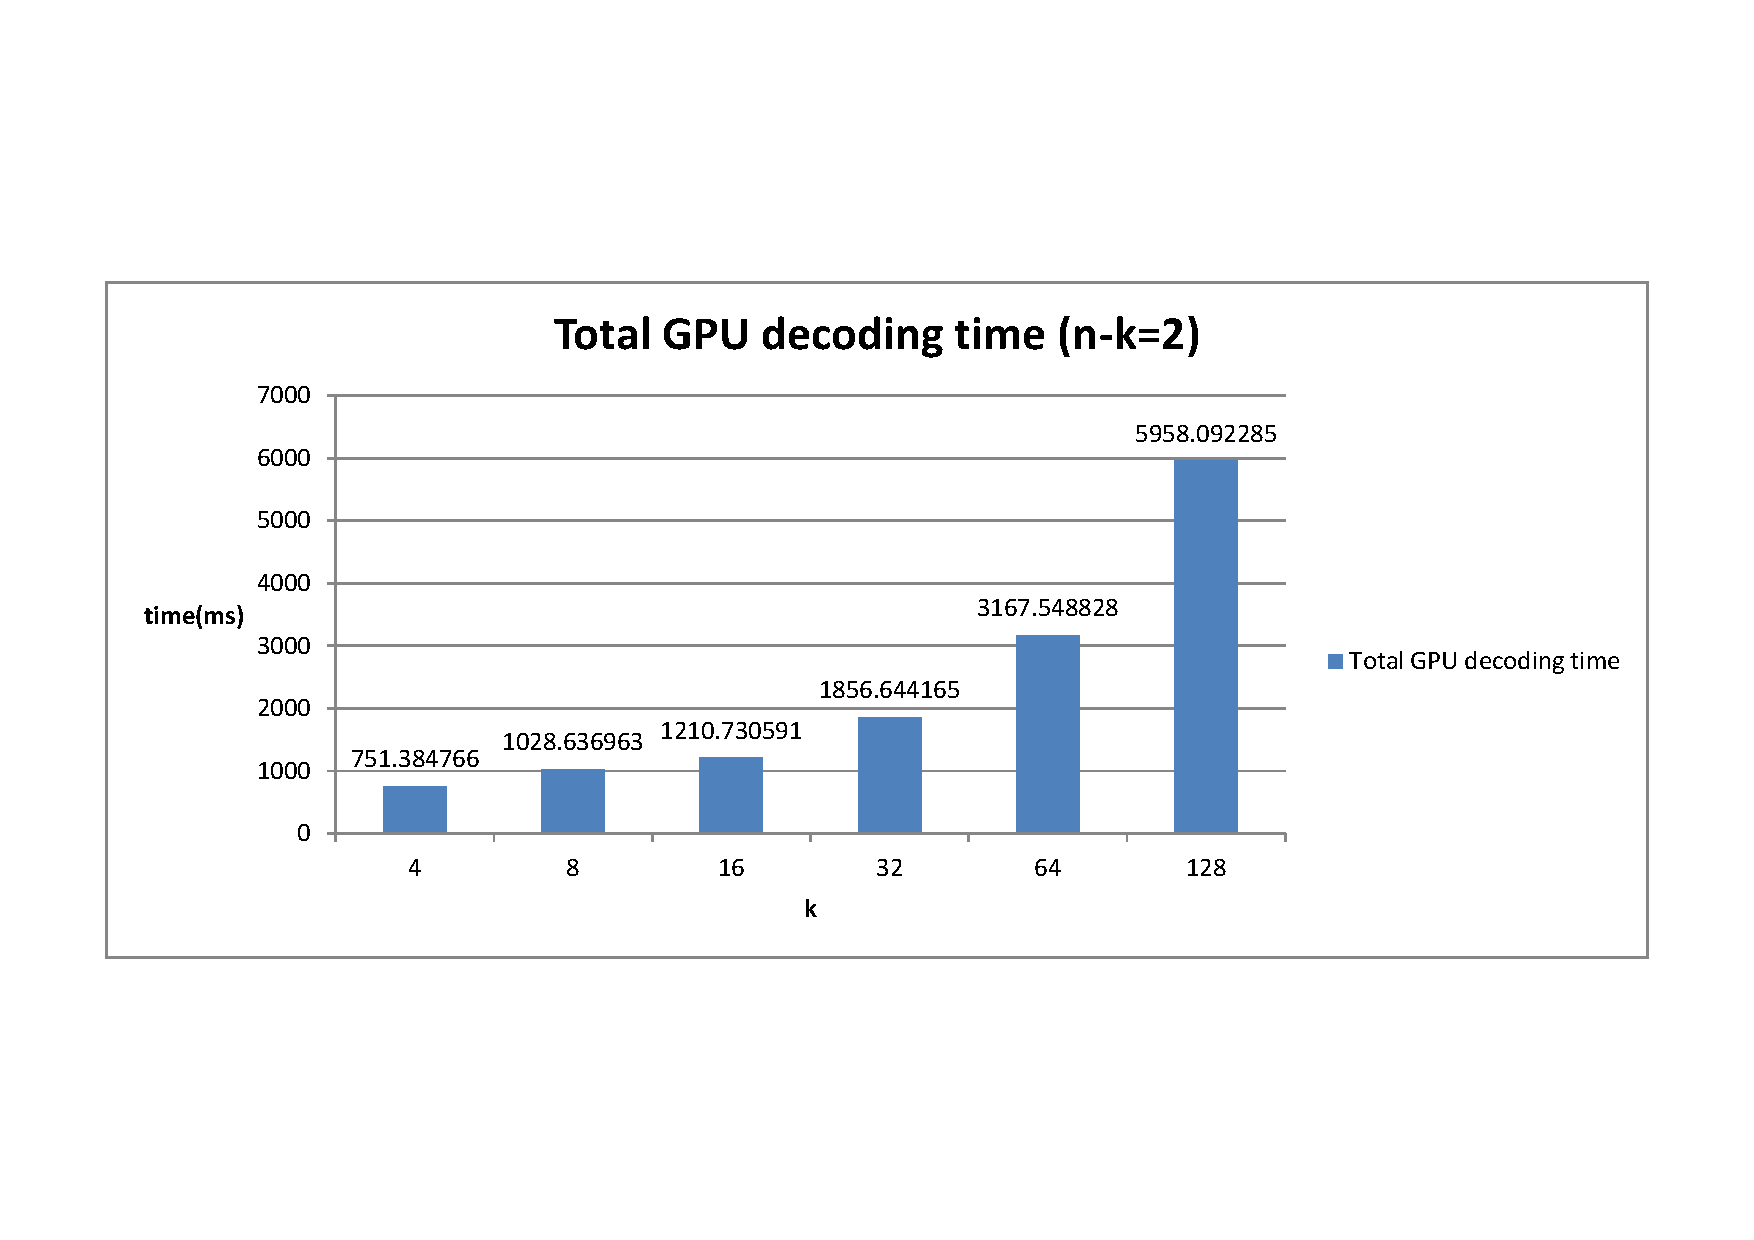
\includegraphics[scale=0.5]{result-graph/Total-GPU-decoding-time-2.pdf}

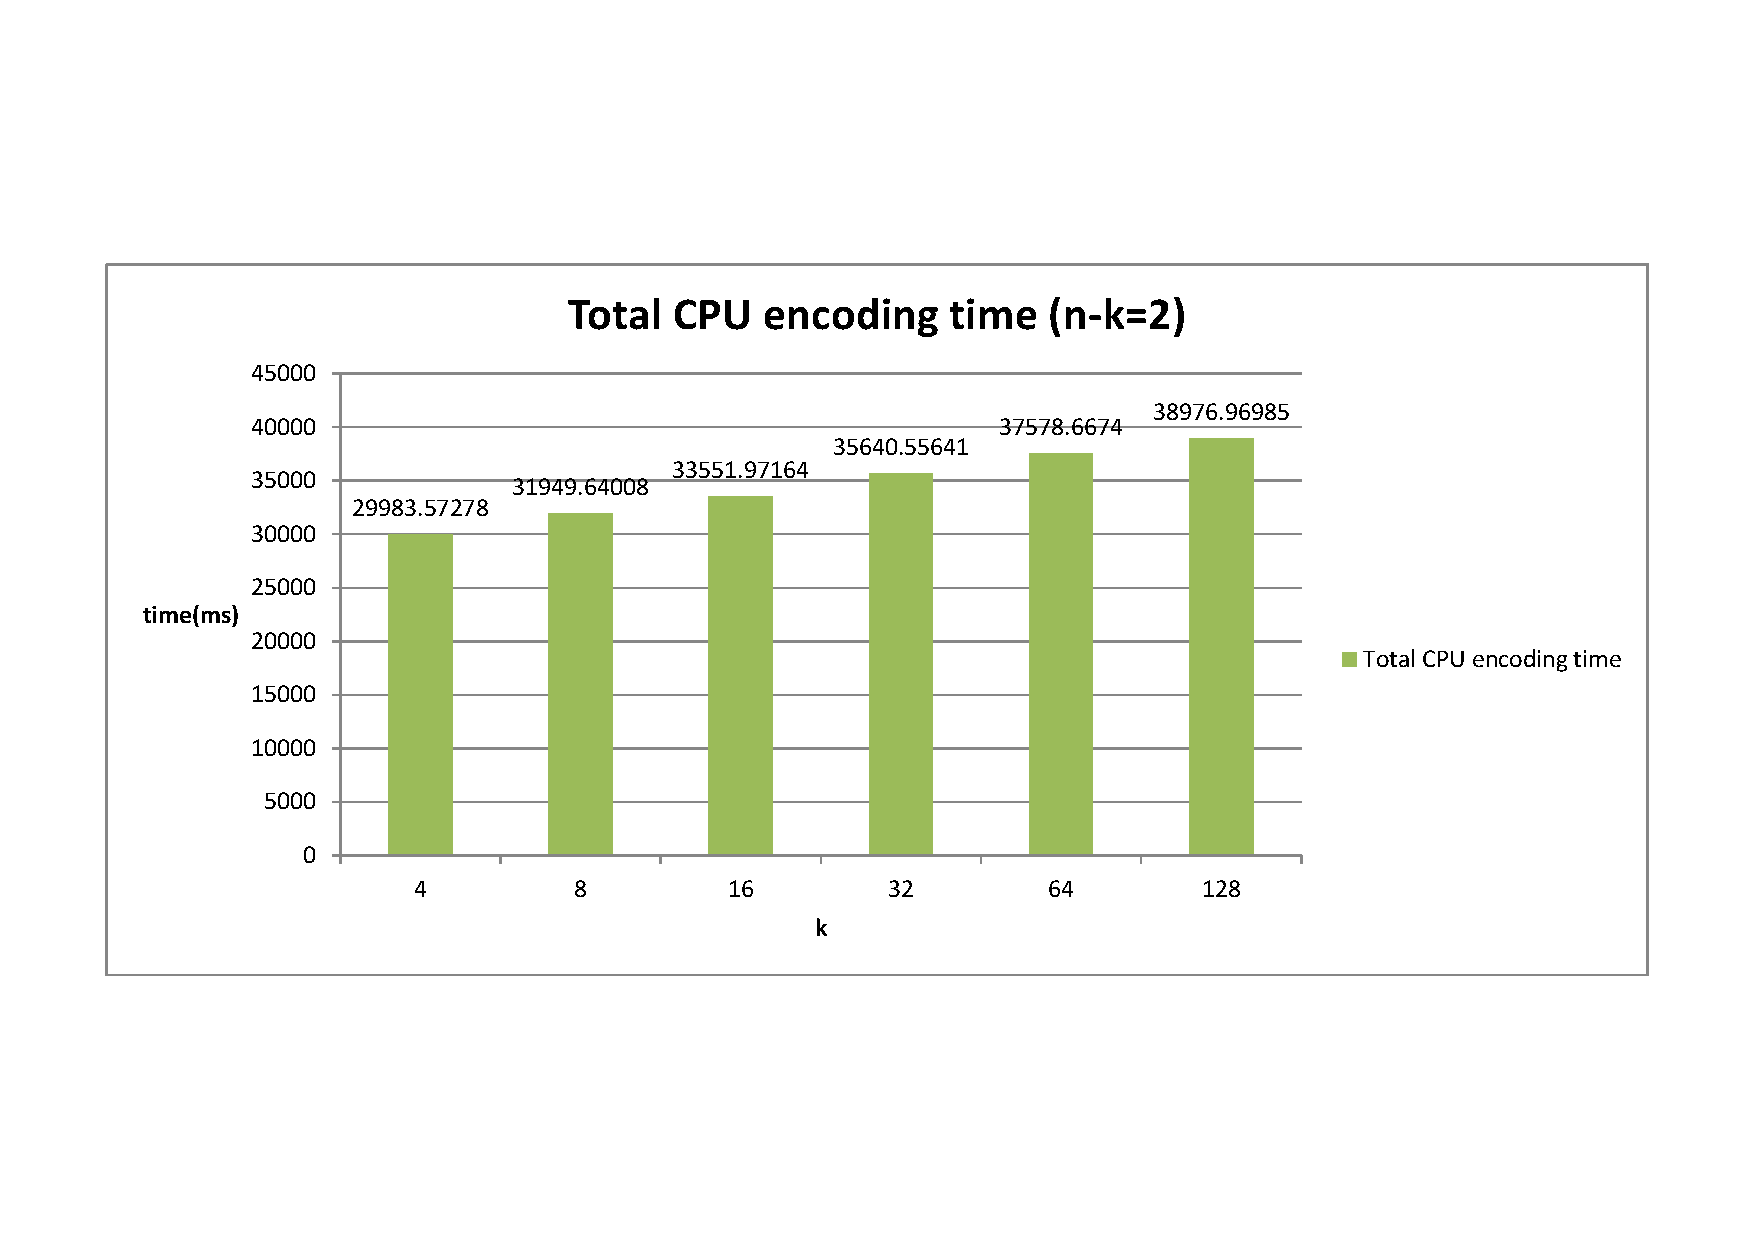
\includegraphics[scale=0.5]{result-graph/Total-CPU-encoding-time-2.pdf}

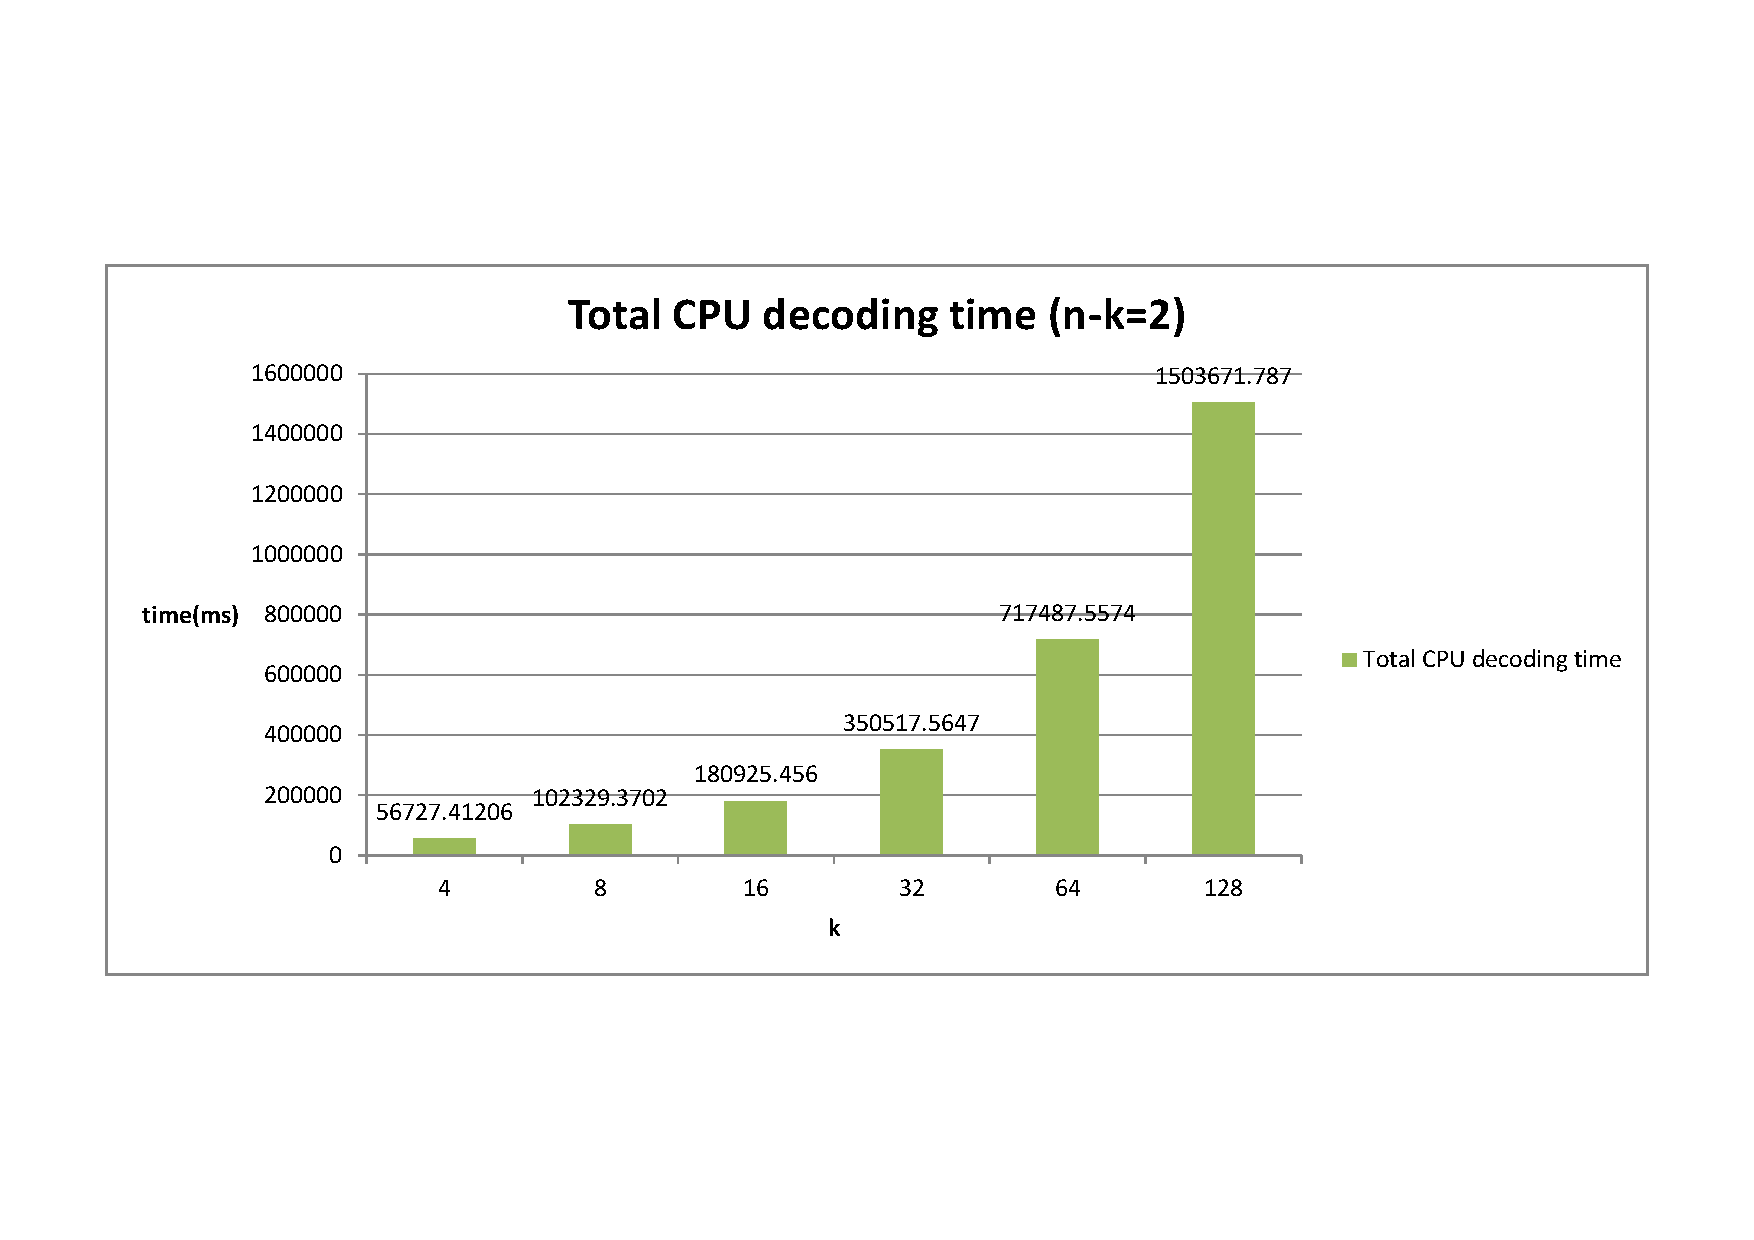
\includegraphics[scale=0.5]{result-graph/Total-CPU-decoding-time-2.pdf}

For triple fault tolerance:

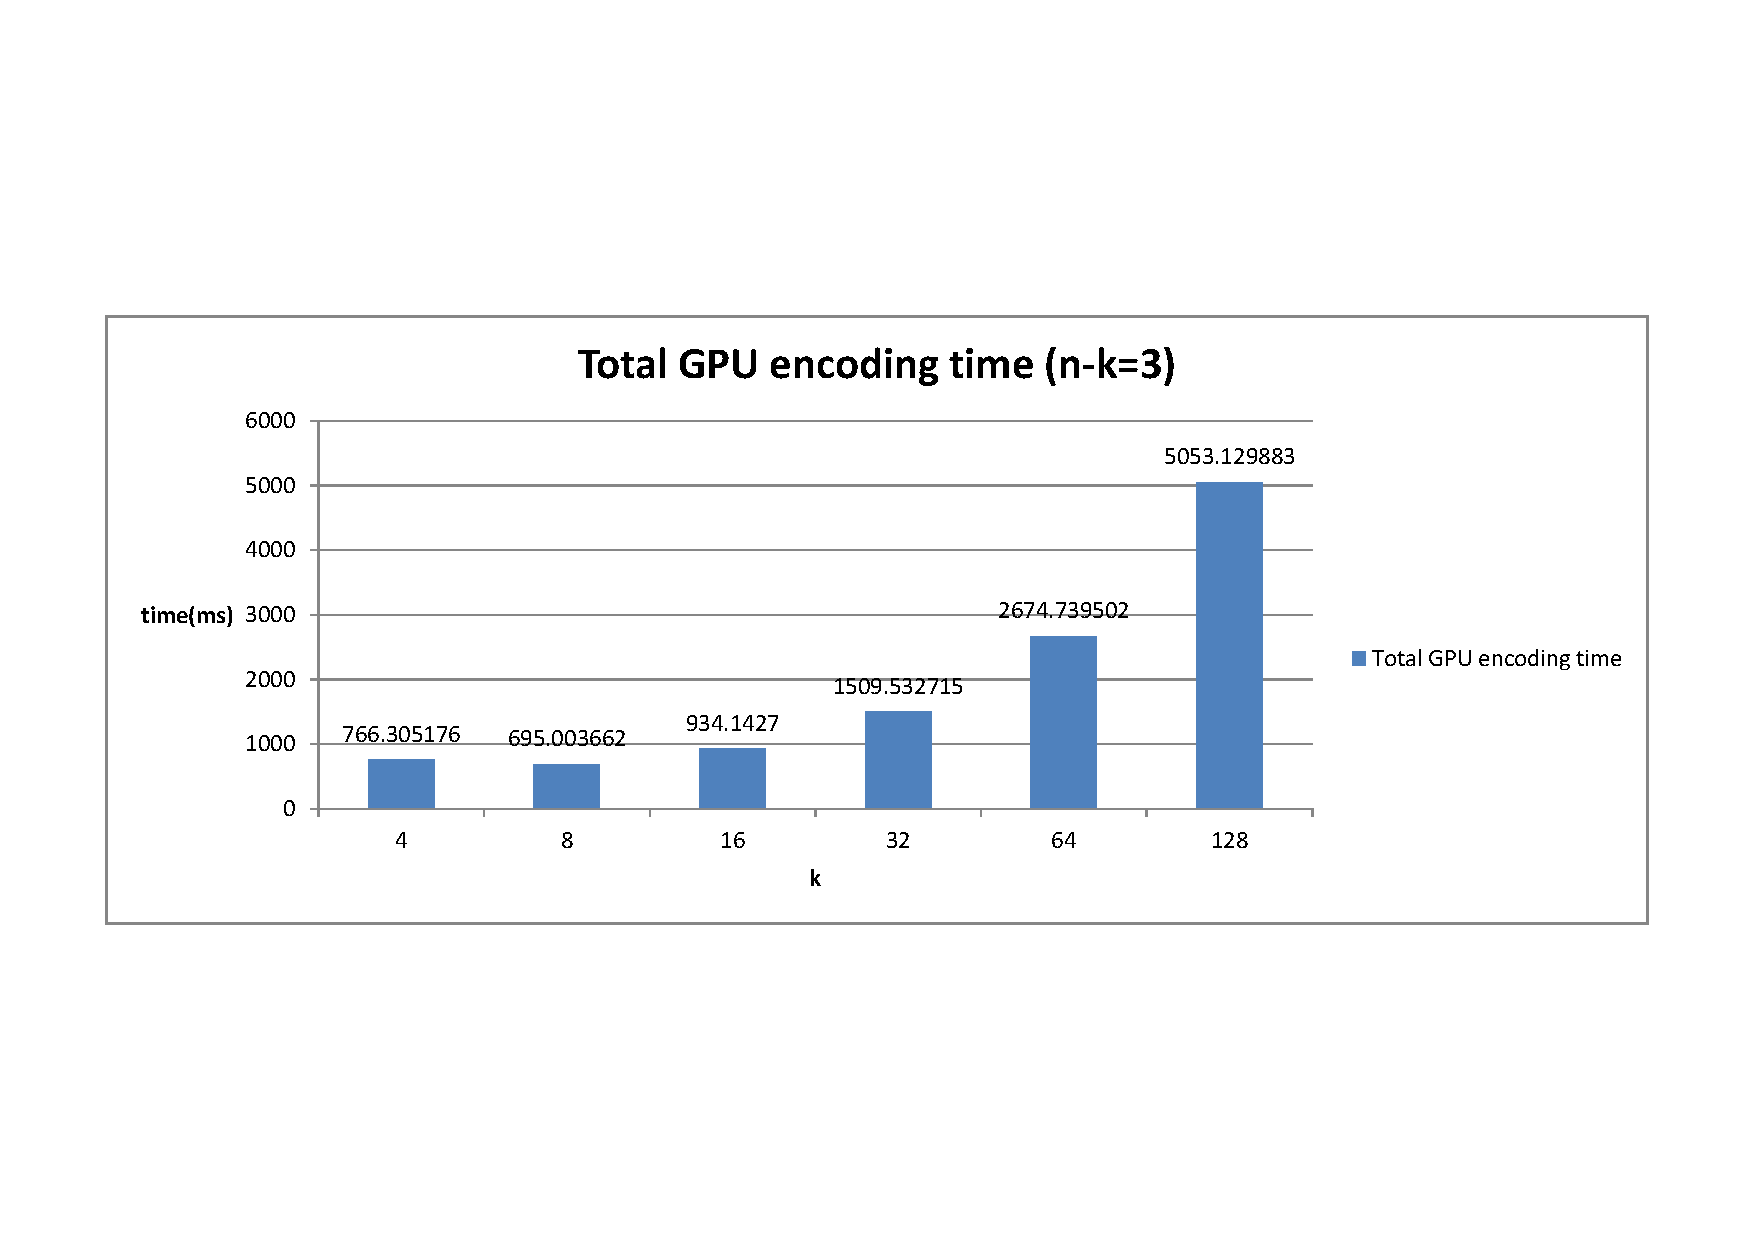
\includegraphics[scale=0.5]{result-graph/Total-GPU-encoding-time-3.pdf}

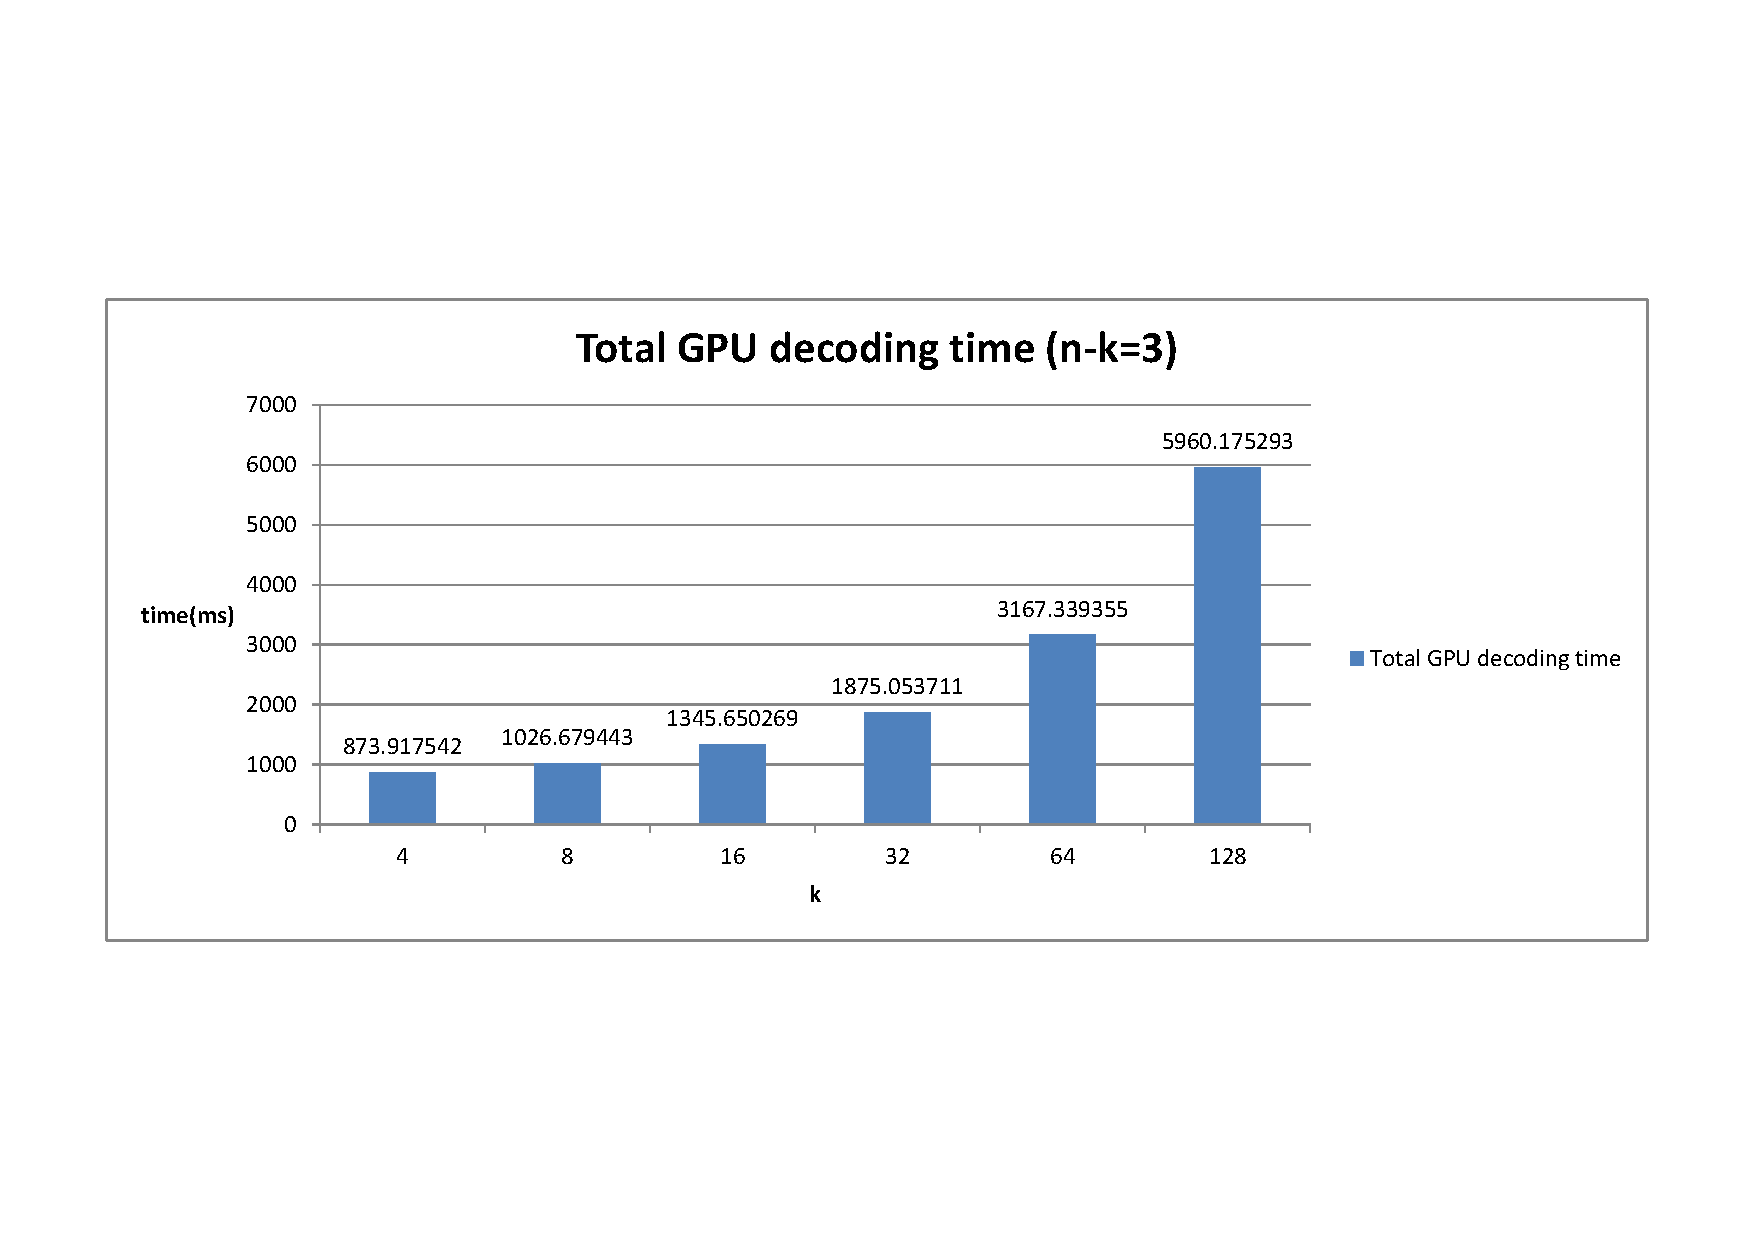
\includegraphics[scale=0.5]{result-graph/Total-GPU-decoding-time-3.pdf}

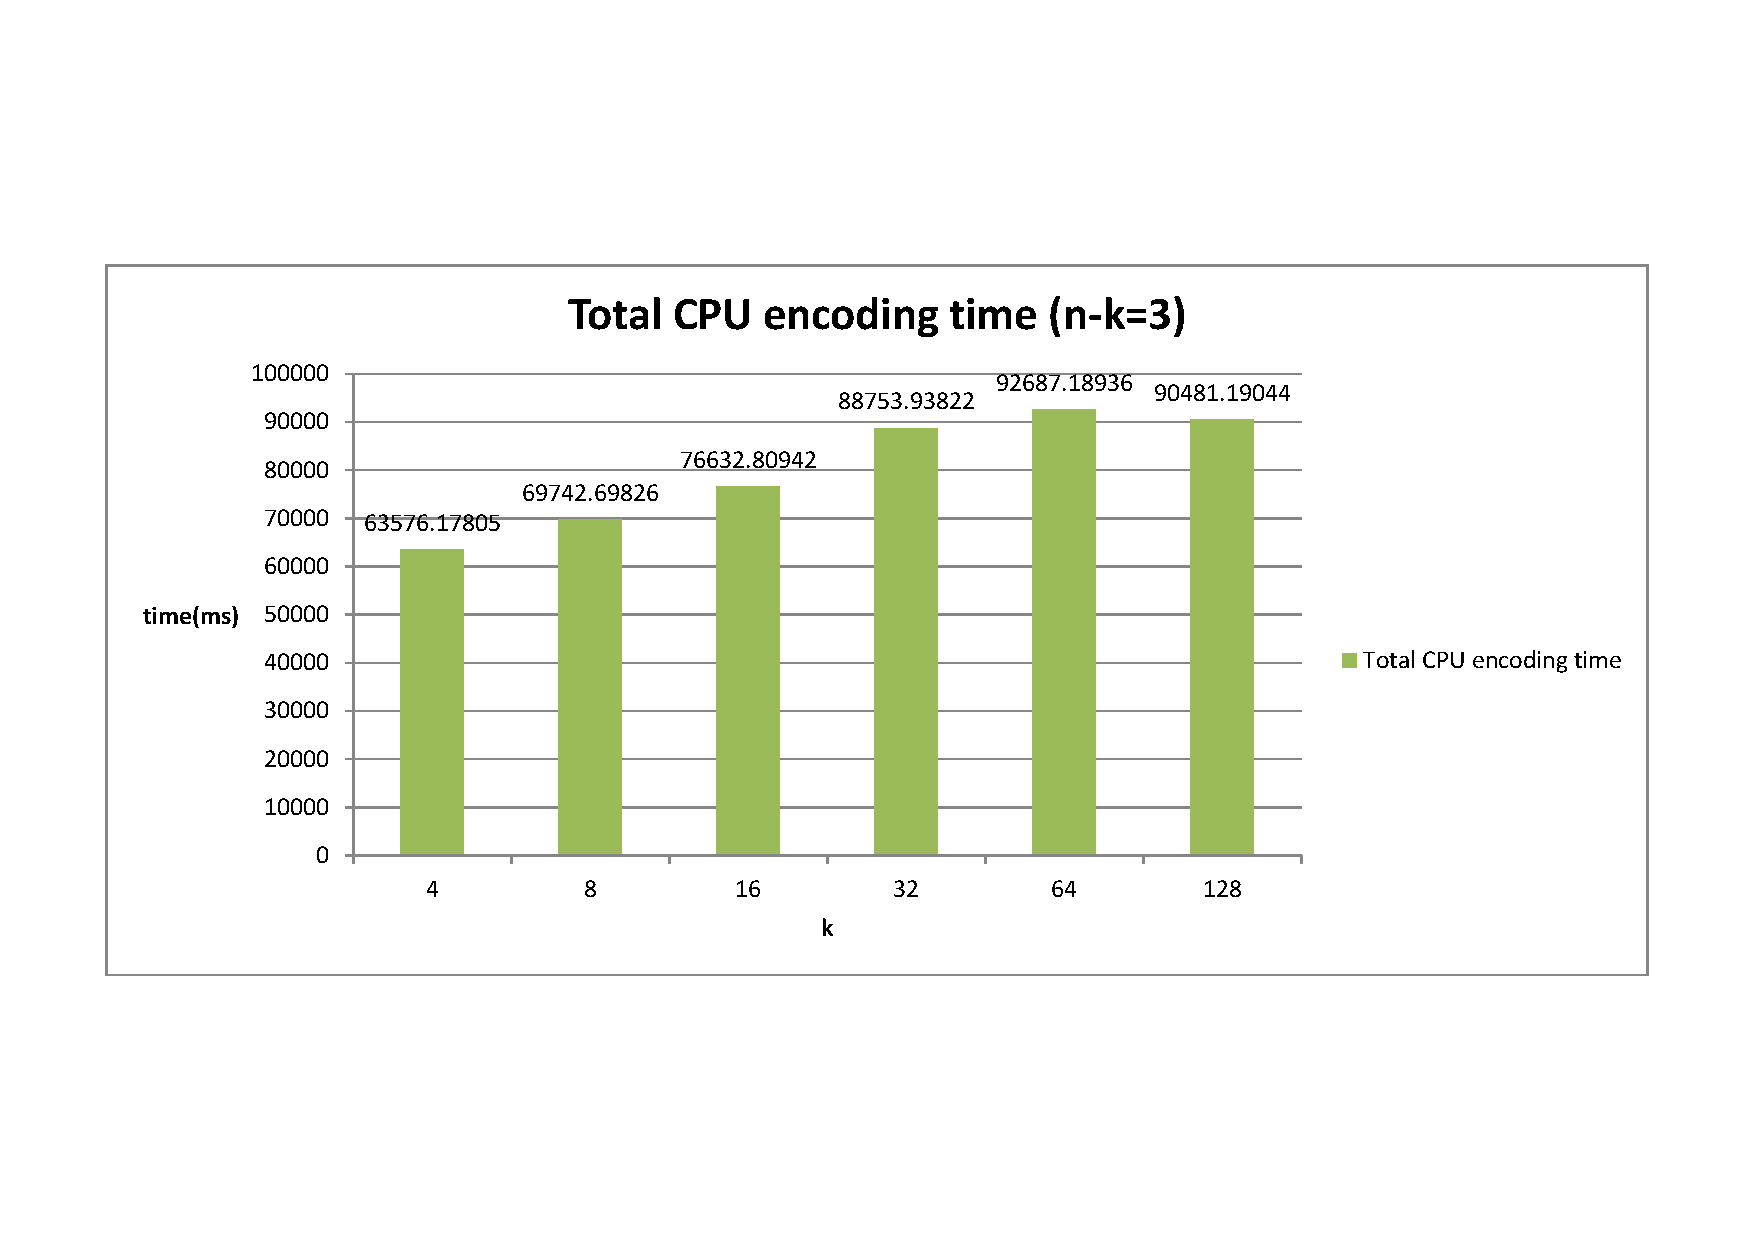
\includegraphics[scale=0.5]{result-graph/Total-CPU-encoding-time-3.pdf}

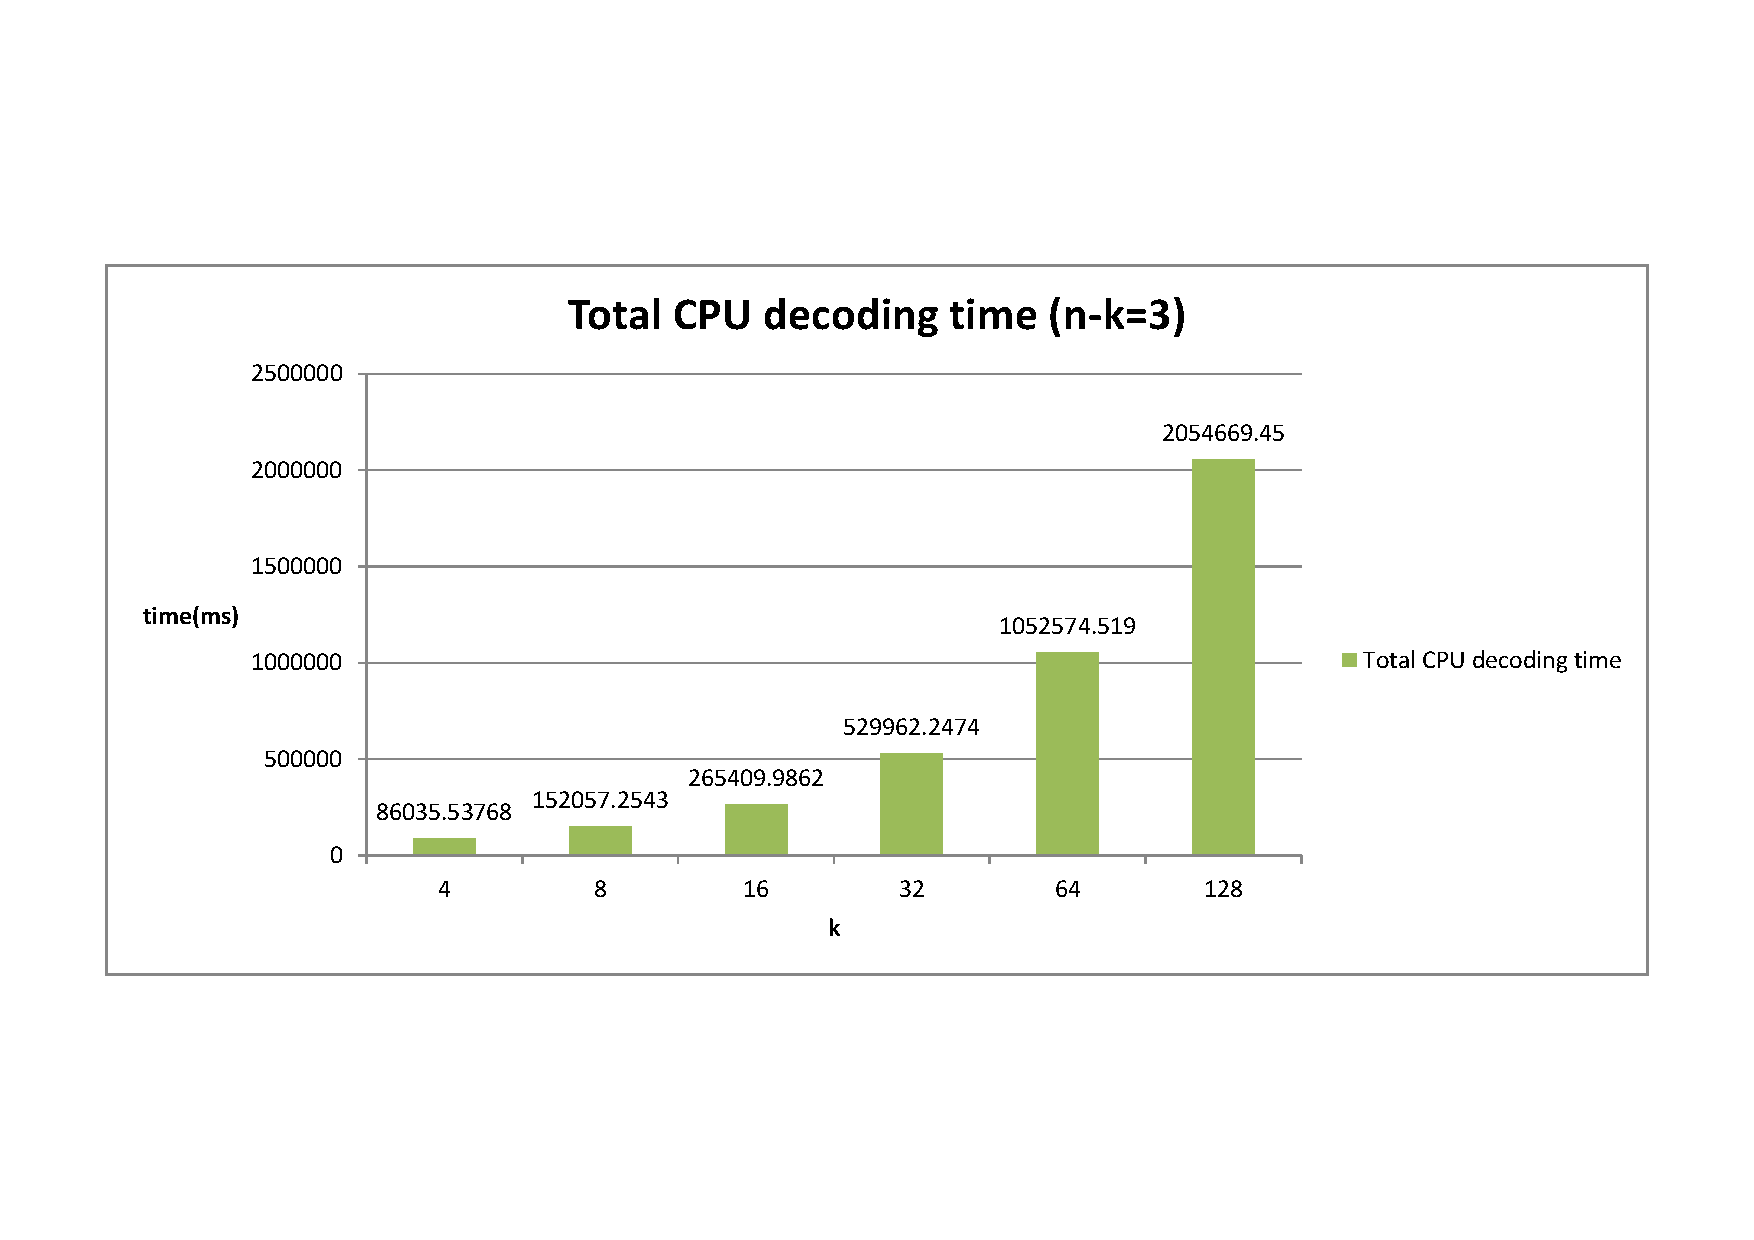
\includegraphics[scale=0.5]{result-graph/Total-CPU-decoding-time-3.pdf}

%We can find in the graphs that the performance of GPU acceleration will be poor if $k$ is no less than 32. But in reality we seldom cut the files into more than 30 fragments, so the overall performance would be still acceptable.
Conclusion:
\begin{enumerate}
\item If we divide the original data into more fragments (i.e. increasing $k$), we can achieve less storage overhead, meanwhile both CPU and GPU performance will become worse.
\item In reality, we seldom cut the files into more than 30 fragments, so the overall performance of GPU would still be acceptable.
\end{enumerate}

\subsection{GF(16) method vs GF(256) method}
In this experiment, we set $k=4, n=6$, and use 1.1GB as file size.

Table \ref{GF16vsGF256} is the performance speed-up of GPU in the Reed-Solomon encoding progress:
\begin{table}
\caption{
GPU cost breakdown comparison between GF(16) and GF(256) methods
}
\begin{center}
\begin{tabular}{|c|c|c|}
\hline
GPU cost breakdown  & GF(16) & GF(256) \\
\hline
Copy data from CPU to GPU(ms)	& 277.482697	& 265.243866 \\
\hline
Generating encoding matrix(ms)	& 0.047328	& 0.252352 \\
\hline
Copy encoding matrix from GPU to CPU(ms)	& 0.023104	& 0.02352 \\
\hline
Encoding file(ms)	& 9.11728	& 160.520676 \\
\hline
copy code from GPU to CPU(ms)	& 193.164154	& 139.608734 \\
\hline
Total computation time(ms)	& 9.164608	& 160.773026 \\
\hline
Total communication time(ms)	& 470.669952	& 404.876129 \\
\hline
Total GPU encoding time(ms)	& 505.69104	& 770.560547 \\
\hline
GPU bandwidth(MB/s)	& 2067.514	& 1356.835 \\
\hline
Copy code from CPU to GPU(ms)	& 276.235229	& 257.23764 \\
\hline
Copy encoding matrix from CPU to GPU(ms)	& 0.013536	& 0.030016 \\
\hline
Generating decoding matrix (inverse matrix)(ms)		& & 1.93504 \\
\hline
Decoding file(ms)	& 16.037184	& 166.371994 \\
\hline
copy data from GPU to CPU(ms)	& 386.210175	& 272.606415 \\
\hline
Total computation time(ms)	& 16.498079	& 168.307037 \\
\hline
Total communication time(ms)	& 662.458984	& 529.874084 \\
\hline
Total GPU decoding time(ms)	& 712.471741	& 731.763733 \\
\hline
GPU bandwidth(MB/s)	& 1467.46	& 1428.772 \\
\hline
\end{tabular}
\label{GF16vsGF256}
\end{center}
\end{table}

Analysis:

For a Galois Field multiplication operation, GF(256) method costs three table-lookups in shared memory (programmable cache in GPU) and one addition and modular in the rational field, while GF(16) costs two table-lookups in constant memory (normally is cached, will costs one additional memory access only on a cache miss) and eight bit-operations ($>>$, $\&$ and $|$).
Thus, the GF(256) method has more communication costs and less computation costs than the GF(16) one.
In the experiment, the GF(16) method is faster in performing matrix multiplication.
However, there is little gap between the overall performance of the two methods.

\section{Future Works}
\begin{itemize}
	\item 
	\item Increase the parallelism of matrix inversion algorithm.
	\item Better CPU/GPU cooperation:								
	\begin{itemize}
		\item 
	\end{itemize}
	\item Implementation Issues:
	\begin{itemize}
		\item While GPU is computing the encoding matrix, CPU can load the input file(s) into memory,
thus making the IO and computation processing roughly at the same time.
	\end{itemize}
\end{itemize}

\section{Appendix}

The source code of this project is available under the GPLv3. And the project's Git repository can be checked out through anonymous access with the following command.
\begin{minted}[frame=lines,mathescape]{bash}
git clone https://github.com/yszheda/GPU-RSCode.git
\end{minted}

The \textbf{master} branch is the implementation of GF(256) Reed-Solomon Code, and the \textbf{extend} is the implementation of GF(16) Reed-Solomon Code, use the following command to checkout one of the branch:
\begin{minted}[frame=lines,mathescape]{bash}
git checkout <branch>
\end{minted}


\bibliographystyle{plain}
\bibliography{design.bib}

%\section{}

\end{document}
